%!TEX TS-program = pdflatexmk

\listfiles
  %%%%%%%%%%%%%%%%%%%%%%%%%%%%%%%%%%%%%%%%%%%%%%%%%%%%%%%%%%%%%%%%%%%%%%%%%%%%%
%%% allgemeine Einstellungen
%%%%%%%%%%%%%%%%%%%%%%%%%%%%%%%%%%%%%%%%%%%%%%%%%%%%%%%%%%%%%%%%%%%%%%%%%%%%%
%\documentclass[twoside,12pt,a4paper]{report}

\documentclass[%
   a4paper,%
 % letterpaper,%
  11pt,                    % alles ein bisschen grˆfler
% twoside,              % Default f¸r scrbook
  openright,              % Kapitel beginnen immer auf der rechten Seite
  %cleardoubleplain, %leere Seite mit plain darstellen - auch cleardoubleempty
  headsepline,          %Linie ¸ber den Kopf
  cleardoubleempty,
  chapterprefix,
  titlepage,%
  liststotoc,%
  bibtotoc,%
  idxtotoc,%
  headinclude,           %will determine if headers and footers are used in the calculation of the page size
%  draft,%
%  final,                    % final ist default
  %BCOR8.25mm,%
  %DIV14,%
  pointlessnumbers,%
  USenglish
  ]{scrbook}

%%%%%%%%%%%%%%%%%%%%%%%%%%
%%% Grafiken
%%%%%%%%%%%%%%%%%%%%%%%%%%

\ifx\pdfoutput\undefined%
  \ExecuteOptions{dvips}
  \usepackage{graphicx}                   % PDF und PNG Graphiken
  \DeclareGraphicsExtensions{.eps.gz,.eps,.ps}
 \else%
  \pdfoutput=1\relax                          % fuer PDF - Compilieren
  \pdfcompresslevel=9                       % fuer PDF - Compilieren
  \ExecuteOptions{pdftex}
  \usepackage{graphicx}                    % PDF und PNG Graphiken
  \DeclareGraphicsExtensions{.pdf,.png,.jpg}
\fi%


\graphicspath{{figures/}{./}}
\newcommand{\FigFB}[2]{\fbox{\includegraphics[#2]{#1}}}
\newcommand{\FigNB}[2]{\includegraphics[#2]{#1}}
\newcommand{\FigFBWide}[1]{%
  \framebox[\textwidth]{\hfill%
    \includegraphics[width=0.98\textwidth]{#1}\hfill}}
\newcommand{\FigNBWide}[1]{\includegraphics[width=\textwidth]{#1}}
\newcommand{\FigFBColumn}[1]{%
  \framebox[\columnwidth]{\hfill%  \DeclareGraphicsRule{.eps.gz}{eps}{.eps.bb}{`gzip -d -c #1}
    \includegraphics[width=0.98\columnwidth]{#1}\hfill}}
\newcommand{\FigNBColumn}[1]{\includegraphics[width=\columnwidth]{#1}}


\def\fcc{\textsc{FeatureC++}\xspace}
\def\fcide{\textsc{FeatureIDE}\xspace}

%%%%%%%%%%%%%%%%%%%%%%%%%%%%%
%%% Zus‰tzliche Pakete
%%%%%%%%%%%%%%%%%%%%%%%%%%%%%
\usepackage[subfigure,titles]{tocloft}
\usepackage{ae,aecompl}                       % CM-Fonts besser
\usepackage[T1]{fontenc}                      % Fontverschl¸sselung
\usepackage[utf8]{inputenc}                 % Umlaute akzeptieren
\usepackage{longtable}
\usepackage{booktabs}													%f¸r optisch schˆne Tabellen
\usepackage[hang,bf,footnotesize,longtable]{caption2}   % bessere Bildunterschriften
\usepackage{parskip}                          % schicke Abs‰tze
%\usepackage{epsf, english}
%\usepackage{english}
%\usepackage{babel}
%\usepackage{supertabular}
%\usepackage[round]{natbib}
\usepackage{afterpage}  % das problem mit den groflen tabellen
\usepackage{url}
\usepackage[sf,sl,outermarks]{titlesec}
\usepackage{color}
\usepackage{amsfonts} %for the display of the |R number space
\usepackage{expdlist} %for nicer lists
\usepackage{listings} %for nicer code display
\usepackage{dsfont}                           % f{\"u}r math. Zahlenbereiche
%\usepackage[hang,footnotesize]{caption2}
\usepackage{graphics}
\usepackage{paralist}
\usepackage{amsmath}
%\usepackage{natbib}
%\bibpunct {[}{]}{;}{a}{,}{,\,}

%\usepackage{graphics}
%\usepackage[pdftex]{graphicx}
%\usepackage[pdftex]{color}
\usepackage{listings}
\usepackage{keyval}
\usepackage[normalem]{ulem}


\usepackage{color}
\usepackage{graphics}
%\usepackage[pdftex]{graphicx}
\usepackage{latexsym}
\usepackage{xspace}
\usepackage{enumitem}
\usepackage{wrapfig}
\usepackage{paralist}
\usepackage{multirow}
\usepackage{placeins}

%\lstset{language=Java,frame=TB,frameround=fftf,basicstyle=\ttfamily \footnotesize,captionpos=b,numbers=left,numberstyle=\tiny,float=float}
%\usepackage{wrapfig}  %fo
%\usepackage[all]{xypic}
%\usepackage{pdftricks}
%\usepackage{amsmath}  %for the display of definitions and such

%\usepackage{AlDraTex}
%\usepackage{TeXProject}

%%%%%%%%%%%%%%%%%%%%%%%%%%%%%%%%%%%%%%%%%%%%%%%%%%%%%%%%%%%%%%%%%%%%
%%%%%%%%%%%%%%%%%%%%%%%%%%%%%%%%%%%%%%%%%%%%%%%%%%%%%%%%%%%%%%%%%%%%
% customization by mleich
%%%%%%%%%%%%%%%%%%%%%%%%%%%%%%%%%%%%%%%%%%%%%%%%%%%%%%%%%%%%%%%%%%%%
\usepackage{tabularx}
\usepackage{longtable}
\usepackage{multirow}

\usepackage{amssymb}

\usepackage{ifthen}
\newboolean{blackandwhitemode}
\newboolean{useinitials}
\newboolean{coloredinitials}

%% -------- CONFIGURE ME! -------- %%
\setboolean{blackandwhitemode}{false}
\setboolean{useinitials}{true}
\setboolean{coloredinitials}{false}
%% -------- CONFIGURE ME! -------- %%

%\typearea[10mm]{12}    % 10mm binding correction, default binding margin is kinda small for uni copyshop
%\areaset[10mm]{157.50mm}{222.75mm}  % areaset version of the above typearea command

\areaset[7mm]{147.50mm}{222.75mm}  % tuned areaset ... good tradeoff between pagewidth and paragraph description margin

\renewcommand{\headfont}{\sffamily\itshape}  % use sans serif italic for page header
%\renewcommand{\pnumfont}{\sffamily\itshape}  % use sans serif italic for page number

% typefaces
\usepackage{palatino}  % Palatino
\usepackage{mathpazo}  % Math Palatino
\usepackage{helvet}    % Helvetica as Sans Serif
\usepackage{microtype} % enable those neat microtype tricks
\usepackage{pdfpages}

\usepackage{textcomp}
\usepackage{varioref}
\usepackage{xfrac}
\usepackage{wrapfig}
\nonfrenchspacing      % grosser Abstand nach Satzende

\usepackage[hang,tight,bf,footnotesize,raggedright]{subfigure}

%% create IEEE cite control command. this would be already there, if we'd be using some IEEE document style
\makeatletter \def\bstctlcite#1{\@bsphack
\@for\@citeb:=#1\do{% \edef\@citeb{\expandafter\@firstofone\@citeb}%
\if@filesw\immediate\write\@auxout{\string\citat ion{\@citeb}}\fi}%
\@esphack} \makeatother

%% mleich's edit helpers
\ifthenelse{\boolean{blackandwhitemode}}{
\definecolor{mleichRed}{cmyk}{0,0,0,1}
\definecolor{mleichBlue}{cmyk}{0,0,0,1}}{
\definecolor{mleichRed}{cmyk}{0,1,1,0}
\definecolor{mleichBlue}{cmyk}{0.9805,0.1299,0,0.4299}}

\newcommand{\MARKED}[2]{\textcolor{#1}{{#2}}}
\newcommand{\TODO}[1]{\message{TODO found!}\MARKED{mleichRed}{TODO-> {#1} <-TODO}}
\newcommand{\CHANGED}[1]{\message{CHANGED found!}\MARKED{mleichBlue}{{#1}}}

% drop capitales / lettrines 
\usepackage{lettrine}
\ifthenelse{\boolean{useinitials}}{
\ifthenelse{\boolean{coloredinitials}}
{\newcommand{\INITIAL}[2]{\lettrine[lines=2,slope=-1pt,nindent=1pt]{\textcolor{mleichRed}{{#1}}}{\textcolor{mleichRed}{{#2}}}}}
{\newcommand{\INITIAL}[2]{\lettrine[lines=2,slope=-1pt,nindent=1pt]{{#1}}{{#2}}}}
}{
\newcommand{\INITIAL}[2]{{#1}{#2}}}

% miscellaneous 
\newcommand{\etal}{et\,al.\ }
\newcommand{\person}[1]{\textsc{#1}}
\newcommand{\ENDSECTION}{\begin{center}
$\spadesuit$
\end{center}
\clearpage}
%%%%%%%%%%%%%%%%%%%%%%%%%%%%%%%%%%%%%%%%%%%%%%%%%%%%%%%%%%%%%%%%%%%%
%%%%%%%%%%%%%%%%%%%%%%%%%%%%%%%%%%%%%%%%%%%%%%%%%%%%%%%%%%%%%%%%%%%%
%%%%%%%%%%%%%%%%%%%%%%%%%%%%%%%%%%%%%%%%%%%%%%%%%%%%%%%%%%%%%%%%%%%%

\lstloadlanguages{Java}
\lstset{basicstyle=\footnotesize,language=Java,tabsize=2,captionpos=b}

%oder: 
%times
%AvantGarde avant 
%NewCentury newcent 
%Helvetica helvet 
%Palatino palatino 
%Bookman bookman 
%Charter charter 
%Utopia utopia

%\usepackage{afterpage}  % das problem mit den groflen tabellen
%\usepackage{reportpage}
%\usepackage{epsf,german}
%\usepackage{latexsym}

%%%%%%%%%%%%%%%%%%%%%%%%%%%%%%%%%%%%%%%%%%
%%% Kapitel-¸berschriften zwischen zwei Linien darstellen:
%%%%%%%%%%%%%%%%%%%%%%%%%%%%%%%%%%%%%%%%%%

\titleformat{\chapter}[display]
  {\normalfont\Large\filcenter\sffamily}
  {\titlerule[1pt]%
   \vspace{1pt}%
   \titlerule
   \vspace{1pc}%
   \LARGE\MakeUppercase{\chaptertitlename} \thechapter}
  {1pc}
  {\titlerule
   \vspace{1pc}%
   \Huge}


\titleformat{\section}
  %{\LARGE\sffamily\slshape}
  {\normalfont\Large\sffamily}
  {\thesection}{1em}{}
 %\titlespacing{\section}
 % {-6pc}{3.5ex plus .1ex minus .2ex}{1.5ex minus .1ex}
 
 \titleformat{\subsection}
  {\normalfont\Large\sffamily}{\thesubsection}{1em}{}
\titleformat{\subsubsection}
  {\normalfont\large\sffamily}{\thesubsubsection}{1em}{}
\titleformat{\paragraph}[runin]
  {\normalfont\normalsize\sffamily}{\theparagraph}{1em}{}
  
\titleformat{\subparagraph}[runin]
  {\normalfont\normalsize\sffamily}{\thesubparagraph}{1em}{}
 

\titleformat{name=\paragraph,page=even}[leftmargin]
 {\sffamily\slshape\filright\footnotesize}
  {}{}{}
\titleformat{name=\paragraph,page=odd}[rightmargin]
 {\sffamily\slshape\filright\footnotesize}
  {}{}{}

\titlespacing{\paragraph}
  {5pc}{1.5ex minus .1 ex}{1pc}
  
  
   
  
  
  
  
  
%%%%%%%%%%%%%%%%%%%%%%%%%%%%%%%%%%%%%%%%%%%%%%%%%%%%%%%%%%%%%%%%%
% XXX
%%%%%%%%%%%%%%%%%%%%%%%%%%%%%%%%%%%%%%%%%%%%%%%%%%%%%%%%%%%%%%%%%
\widowpenalty 10000                           % Keine Hurenkinder
\displaywidowpenalty 10000                    % Keine Hurenkinder (Formeln)
\clubpenalty 10000                            % Keine Schusterjungen

%%%%%%%%%%%%%%%%%%%%%%%%%%%%%%%%%%%%%%%%%%%%%%%%%%%%%%%%%%%%%%%%
% Captions f¸r Tables in Subfigures oder umgekehrt
%%%%%%%%%%%%%%%%%%%%%%%%%%%%%%%%%%%%%%%%%%%%%%%%%%%%%%%%%%%%%%%%
\makeatletter
\newcommand\tabcaption{\def\@captype{table}\caption}
\newcommand\figcaption{\def\@captype{figure}\caption}
\makeatother
  
%%%%%%%%%%%%%%%%%%%%%%%%%%%%%%%%%%%%%%%%%%%%%%%%%%%%%%%%%%%%%%%%%
% Fussnote neu definieren (links und rechts ausgeglichen)
%%%%%%%%%%%%%%%%%%%%%%%%%%%%%%%%%%%%%%%%%%%%%%%%%%%%%%%%%%%%%%%%%
\newlength{\fnnumwidth}\setlength{\fnnumwidth}{1.5em}
\newlength{\fntextwidth}\setlength{\fntextwidth}{\textwidth}
\addtolength{\fntextwidth}{-1.5em}
\makeatletter
\renewcommand{\@makefntext}[1]{%
         \noindent\begin{minipage}[t]{\fnnumwidth}%
           \@thefnmark %
         \end{minipage}%
         \begin{minipage}[t]{\fntextwidth}%
         {#1}%
         \end{minipage}%
}
\makeatother


\definecolor{grey}{cmyk}{0.0,0.0,0.0,0.075}

\setlength{\parskip}{0cm}

\lstdefinelanguage{fc++}[ANSI]{c++}%
  {morekeywords={refines,super,this,layer},%
   sensitive=f
   }[keywords,comments,strings]%

\lstdefinelanguage{afc++}[ANSI]{c++}%
  {morekeywords={refines,super,this,layer,pointcut,call,aspect, template},%
   sensitive=f
   }[keywords,comments,strings]%

\lstset{basicstyle=\tt\tiny,
	keywordstyle=\tt\tiny\bf,
	commentstyle=\tt\tiny\it,
	escapechar=,
	tabsize=2,
	language=java,
	numbers=left,
	firstline=1,
	framexleftmargin=0mm,
	frame=left|right|bottom|top,
	rulesepcolor=\color{black},
	backgroundcolor=\color{grey}
}

%%%%%%%%%%%%%%%%%%%%%%%%%%%%%%%%%%%%%%%%%%%%%%%%%%%%%%%%%%
% Inhaltsverzeichnis mit Strich unter Chapter
%%%%%%%%%%%%%%%%%%%%%%%%%%%%%%%%%%%%%%%%%%%%%%%%%%%%%%%%%%
\makeatletter
%Gliederungsnummer
\renewcommand{\numberline}[1]{%
  \makebox[0.9cm][l]{#1}\hspace{1mm}}
  
%chapter
\renewcommand{\l@chapter}[2]{%
  \addvspace{2ex}%                       vert. Abstand
  \pagebreak[3]%                         Seitenumbruch hier erlauben
  \noindent%                             nicht einr¸cken
  \makebox[0pt][l]{%                     Box f¸r Linie
     \rule[-3pt]{.93\textwidth}{0.5pt}}%    Linie f¸r Textbreite
     {\large\textbf{#1}}\hfill#2%        Text + Nummer
     \par%                               Zeilenumbruch
     \nopagebreak%                       Seitenumbruch nicht erlauben
     \addvspace{1ex}%                    vert. Abstand
}
%section
\renewcommand{\l@section}[2]{%
  \addvspace{0.5ex}%                     vert. Abstand
  \noindent\hspace{1cm}%                 hor. Einr¸cken 2em
  #1\hfill#2%                            Text + Nummer
  \par%                                  Zeilenumbruch
  \nopagebreak[2]%                       mˆglichst keinen Seitenumbruch
}

%subsection
\renewcommand{\l@subsection}[2]{%
  \addvspace{0.2ex}%                     vert. Abstand
  \noindent\hspace{2cm}%                 hor. Einr¸cken 5em
  #1\hfill#2%                           Text+Nummer
  \par%                                  Zeilenumbruch
}
\makeatother
     

%%%%%%%%%%%%%%%%%%%%%%%%%%%%%%%
%%% Zus‰tzliche Kommandos
%%%%%%%%%%%%%%%%%%%%%%%%%%%%%%%
\newcommand{\mparQ}[1]{[\textcolor{red}{\textbf{?}}\marginpar{\textcolor{red}{#1 ?}}]}
\newcommand{\mparA}[1]{[\textcolor{red}{\textbf{!}}\marginpar{\textcolor{red}{#1 !}}]}
\newcommand{\mparT}[1]{[\textcolor{blue}{\textbf{T}}\marginpar{\textcolor{blue}{Tabelle \scriptsize{#1}}}]}

\newcommand{\project}[1]{\textit{#1}}

\renewcommand{\baselinestretch}{1.2}\normalsize
\newcommand{\vs}[0]{\vspace{1em}}

\newlength{\pictureheight}
\newlength{\picturewidth}
\newlength{\picturesep}


%%%%%%%%%%%%%%%%%%%%%%%%%%%%%%%%%%%%%%%HIER
%\textwidth 15.8cm
%\textheight 22cm
%\headsep 3em
%\headheight 1em
%\evensidemargin -0.5cm
%\oddsidemargin 1cm


%%% Die Listenumgebung ‰ndern
%%%%%%%%%%%%%%%%%%%%%%%%%%%%%%%%%%
\renewcommand{\labelitemi}{$\circ$} %(erste Ebene)


%%%%%%%%%%%%%%%%%%%%%%%%%%%%%%%%%%
%%% Das Problem mit den subfigures
%%%%%%%%%%%%%%%%%%%%%%%%%%%%%%%%%%
%\newbox\subfigbox %Create a box to hold a subfigure
%\makeatletter
%  \newenvironment{subfloat}% % Create the new environment
%     {\def\caption##1{\gdef\subcapsave{\relax##1}}%
%      \let\subcapsave=\@empty %save the subcaption text
%      \let\sf@oldlabel=\label
%      \def\label##1{\xdef\sublabsave{\noexpand\label{##1}}}%
%      \let\sublabsave\relax %save the label key.
%      \setbox\subfigbox\hbox
%       \bgroup}%     %open the box
%       {\egroup      %...close the box and call \subfigure
%       \let\label=\sf@oldlabel
%       \subfigure[\subcapsave]{\box\subfigbox}}%
% \makeatother

%%%%%%%%%%%%%%%%%%%%%%%%%%%%%
%%% F¸r PDF
%%%%%%%%%%%%%%%%%%%%%%%%%%%%%
% ----------------------------------------------------------
% Einstellungen zu Hyperref,
% z.B. Document-Description-Felder in der PDF-Datei
% MUSS AM SCHLUSS DER PRAEAMBEL STEHEN!
% ----------------------------------------------------------
\usepackage{hyperref}

\hypersetup{
  pdfcreator={LaTeX2e},
  plainpages=false,       % For problems with page referencing
  hypertexnames=false,    % For handling subfigures correctly
  bookmarks=true,         % I want bookmarks
  bookmarksnumbered=false,% Include the section numbers in the list
  bookmarksopen=true,     % In the list, display highest level only
  bookmarksopenlevel=3,   % Display three levels of bookmarks
  pdfpagemode=UseNone,    % Show just the page
  pdfstartview=Fit,
  pdfborder=0,            % I don't want those silly boxes
  breaklinks=true,        % Allow breaking links
  colorlinks=false,		 % Don't change coloring of links
  pdftitle={TODO: INSERT PDF TITLE},
  pdfauthor={PDF AUTHORNAME},
  pdfsubject={PDF SUBJECT}
  }       

\ifx\pdfoutput\undefined%
  \renewcommand{\pdfbookmark}[3][]{}
\fi%

%%%%%%%%%%%%%%%%%%%%%%%%%%%%%%%%%%%%%%%%%%%%%%%%%
% F¸r die Mathematik
%%%%%%%%%%%%%%%%%%%%%%%%%%%%%%%%%%%%%%%%%%%%%%%%%
\usepackage[hyperref]{ntheorem}
\theoremlisttype{allname}
%\setlength{\theoremindent}{1cm}
\newtheorem{lemma}{Lemma}[chapter]
\newtheorem{definition}{Definition}[chapter]
\theoremstyle{break}
\theoremseparator{:}
\setlength{\theorempreskipamount}{2ex plus0.5ex minus0.5ex}
\setlength{\theorempostskipamount}{0.5ex plus0.5ex minus0.5ex}
\newtheorem{proposition}{Proposition}





\begin{document}


%%%%%%%%%%%%%%%%%%%%%%%%%%%%%%%%%%%%%%%%%%%%%%%%%%%%%%%%%%%%%%%%%%%%%%%%%%%%
%%% hier steht die neue Titelseite
%%%%%%%%%%%%%%%%%%%%%%%%%%%%%%%%%%%%%%%%%%%%%%%%%%%%%%%%%%%%%%%%%%%%%%%%%%%%
\begin{titlepage}
    \begin{center}
        \vspace*{1cm}
        
        \Huge
        \textbf{Visualization of Data Flow Graphs for In Situ Data Analysis}
        
        \vspace{0.5cm}
        \LARGE
        %Thesis Subtitle
        
        \vspace{1.5cm}
        
        \textbf{Jacob Edwards}
        
        \vfill
        
        A thesis presented for the degree of\\
        Master of Science
        
        \vspace{0.8cm}
        
        
\includegraphics[width=0.3\textwidth]{tub_logo.png}
        
        \Large
        Database Systems and Information Management Group\\
        Technische Universität Berlin\\
        Berlin, Germany\\
        31/07/2015
        
    \end{center}
\end{titlepage}

%%%%%%%%%%%%%%%%%%%%%%%%%%%%%%%%%%%%%%%%%%%%%%%%%%%%%%%%%%%%%%%%%%%%%%%%%%%%
%%% Titelr¸ckseite: Bibliographische Angaben
%%%%%%%%%%%%%%%%%%%%%%%%%%%%%%%%%%%%%%%%%%%%%%%%%%%%%%%%%%%%%%%%%%%%%%%%%%%%

\vspace*{\fill}
\begin{minipage}{15cm}
\textbf{Author:}\\
\emph{Jacob Edwards}\\Technische Universität Berlin\\
Berlin, 2015.
\end{minipage}
\newpage

%%%%%%%%%%%%%%%%%%%%%%%%%%%%%%%%%%%%%%%%%%%%%%%%%%%%%%%%%%%%%%%%%%%%%%%%%%%%
%%% Kopie der Aufgabenstellung
%%%%%%%%%%%%%%%%%%%%%%%%%%%%%%%%%%%%%%%%%%%%%%%%%%%%%%%%%%%%%%%%%%%%%%%%%%%%


\thispagestyle{empty}
\pdfbookmark{Abstract}{abstract}
%% Zusammenfassung in Englisch
\begin{center}
\textbf{Abstract}
\end{center}

\paragraph{}
The aim of this work is to research suitable visualization techniques for application in data flow graph based analysis systems. To accomplish this, a literature survey was performed over the relevant works in the fields of both visualization and data analysis platforms. An examination of appropriate matches between analysis tasks and visualization techniques was performed, from which a prototypical visualization system for use in analysis scenarios was developed.

\paragraph{}
Several application scenarios are examined using the developed visualization system, and a discussion of the value of visualization in each scenario is given. Finally, implementation details of the visualization framework and potential areas for future improvement are given.

\ \\

\begin{center}
\textbf{Zusammenfassung}
\end{center}

\paragraph{}
Das Ziel dieser Arbeit ist es, geeignete Visualisierungstechniken für den Einsatz in Datenflussgraphen basierend Analysesysteme zu erforschen. Um dies zu erreichen, wurde eine Literaturrecherche in den relevanten Arbeiten auf den Gebieten der beiden Visualisierung und Datenanalyse-Plattformen durchgeführt. Eine Untersuchung der entsprechenden Übereinstimmungen zwischen Analyseaufgaben und Visualisierungstechniken durchgeführt wurde, aus dem eine protoVisualisierungsSystem zur Verwendung in Analyseszenarios entwickelt wurde.

\paragraph{}
Verschiedene Anwendungsszenarien werden unter Verwendung der entwickelten Visualisierungssystem untersucht, und eine Diskussion über den Wert der Visualisierung in jedem Szenario ist gegeben. Schließlich werden Implementierungsdetails der Visualisierungs-Framework und potenzielle Bereiche für künftige Verbesserungen gegeben.

\bigskip

\newpage

\thispagestyle{empty}
\pdfbookmark{Acknowledgements}{conform}
\begin{center}
\textbf{Acknowledgements}
\end{center}

\newpage



%%%%%%%%%%%%%%%%%%%%%%%%%%%%%%%%%%%%%%%%%%%%%%%%%%%%%%%%%%%%%%%%%%%%%%%%%%%%
%%% Rˆmische Seitennumerierung beginnend mit 1
%%%%%%%%%%%%%%%%%%%%%%%%%%%%%%%%%%%%%%%%%%%%%%%%%%%%%%%%%%%%%%%%%%%%%%%%%%%%

\pagenumbering{roman}
\setcounter{page}{1}

%%%%%%%%%%%%%%%%%%%%%%%%%%%%%%%%%%%%%%%%%%%%%%%%%%%%%%%%%%%%%%%%%%%%%%%%%%%%%
%%% Inhaltsverzeichnis
%%%%%%%%%%%%%%%%%%%%%%%%%%%%%%%%%%%%%%%%%%%%%%%%%%%%%%%%%%%%%%%%%%%%%%%%%%%%%

%\renewcommand{\baselinestretch}{1.3}
%\small\normalsize

\pdfbookmark{Table of Contents}{tableofcontents}
\tableofcontents
%\renewcommand{\baselinestretch}{1}
%\small\normalsize

\cleardoublepage

%%%%%%%%%%%%%%%%%%%%%%%%%%%%%%%%%%%%%%%%%%%%%%%%%%%%%%%%%%%%%%%%%%%%%%%%%%%%%
%%% Abbildungsverzeichnis
%%%%%%%%%%%%%%%%%%%%%%%%%%%%%%%%%%%%%%%%%%%%%%%%%%%%%%%%%%%%%%%%%%%%%%%%%%%%%

%\renewcommand{\baselinestretch}{1.3}
%\small\normalsize

\setlength{\cftfignumwidth}{1cm}
\listoffigures
%\addcontentsline{toc}{chapter}{List of Figures}

%\renewcommand{\baselinestretch}{1}
%\small\normalsize

\cleardoublepage

%%%%%%%%%%%%%%%%%%%%%%%%%%%%%%%%%%%%%%%%%%%%%%%%%%%%%%%%%%%%%%%%%%%%%%%%%%%%%
%%% Tabellenverzeichnis
%%%%%%%%%%%%%%%%%%%%%%%%%%%%%%%%%%%%%%%%%%%%%%%%%%%%%%%%%%%%%%%%%%%%%%%%%%%%%

%\renewcommand{\baselinestretch}{1.3}
%\small\normalsize

%\listoftables
%\addcontentsline{toc}{chapter}{List Of Tables}

%\renewcommand{\baselinestretch}{1}
%\small\normalsize

%\cleardoublepage

%%%%%%%%%%%%%%%%%%%%%%%%%%%%%%%%%%%%%%%%%%%%%%%%%%%%%%%%%%%%%%%%%%%%%%%%%%%%%
%%% Abk¸rzungsverzeichnis
%%%%%%%%%%%%%%%%%%%%%%%%%%%%%%%%%%%%%%%%%%%%%%%%%%%%%%%%%%%%%%%%%%%%%%%%%%%%%

\chapter*{List of Abbreviations}
\addcontentsline{toc}{chapter}{List of Abbreviations}

\begin{tabbing}
\textbf{FACTOTUM}\hspace{1cm}\=Schrott\kill
\textbf{DAG}\>directed acyclic graph\\
\textbf{KPI}\>key performance indicator\\
\end{tabbing}


\cleardoublepage

%%%%%%%%%%%%%%%%%%%%%%%%%%%%%%%%%%%%%%%%%%%%%%%%%%%%%%%%%%%%%%%%%%%%%%%%%%%%%
%%% Der Haupttext, ab hier mit arabischer Numerierung
%%% Mit \input{dateiname} wird die Datei `dateiname' eingebunden
%%%%%%%%%%%%%%%%%%%%%%%%%%%%%%%%%%%%%%%%%%%%%%%%%%%%%%%%%%%%%%%%%%%%%%%%%%%%%

\pagenumbering{arabic}
\setcounter{page}{1}

%\chapter*{Test}
%\addcontentsline{toc}{chapter}{Test}

\chapter{Introduction}
\label{sec:Introduction}



\section{Motivation}
\INITIAL{I}{n-situ} data processing is currently extremely popular. In this approach, in order to achieve the minimum possible time in which results are returned, very little preprocessing of any kind is performed. This means that users do not have a very comprehensive understanding of the nuances and problems which may exist in the data beforehand. Any potential pitfalls are likely to only be discovered at a later time, after much time and effort will already have been invested.

\paragraph{Intermediate data sets}
Standard statistics such as minimum, maximum, average, or median may help for simple numeric data. However, text data or (semi-) structured data call for different approaches. Aside from knowing what your raw data looks like at the input stage it is also crucial to understand intermediate data sets, i.e. how the different operations affect the data within the data flow.

\paragraph{Directed Acyclic Graphs}
It is typical for large scale analysis systems such as Flink \cite{Battre2010}, Pig \cite{Gates2009}, or IBMs System S \cite{Gedik2008} to represent analysis jobs as a series of individual tasks. These tasks are connected into a data flow which generally takes the form of an directed acyclic graph (DAG), which provides a useful visual metaphor for the ordering and dependencies of each task within a job. While this is adequate for describing the process by which data is analyzed, it leaves much to be desired in terms of describing the data itself. In particular, in cases where execution times are particularly long. Thus far, few systems making use of data flow graphs have invested significantly in the area of visual feedback within these graphs. System S provides basic feedback indicating the status of dataset processing without real feedback regarding data features \cite{Pauw2010}, and Lipstick \cite{Amsterdamer2011} has evolved from a method of providing provenance models for pig latin queries to providing rudimentary DAG visualization capabilities for Apache Pig \cite{Gates2009} in its current development state.

\paragraph{Data Set Visualizations}
The purpose of this work is to research suitable visualization techniques for a wide array of common analysis tasks, survey the relevant literature, and create a prototypical method for the implementation of these visualizations in a data flow context. These visualizations are proposed in such a way as to be generic enough to suit many types of analysis without modification, and to demonstrate the effects of different operations on the data as well as interesting traits which are inherent to the input data sets in their raw state. Necessarily, to demonstrate this an examination of both common visualizations as well as common analysis tasks are presented, after which the applications of both together are demonstrated and discussed on some representative samples. Additionally, cases where such a solution is either inappropriate or ineffective without modification are presented.

\paragraph{Scope of Work}
Though this work aims to be comprehensive, there is of course a limit to the topics which have been addressed. In particular, focus has been placed squarely on the visualization of data sets as they are processed through a data flow; meaning that input, output, and intermediate data sets are discussed but the visualization of the data flow graphs themselves has been omitted. This is due to the relatively extensive work that has already been done to address this facet of data flow visualization. Additionally, as this work is intended to be prototypical there are some clearly beneficial features which have not been implemented thus far. Principle among these features is automation of the visualization process, which in its current form requires explicit action on the part of developers. Additionally, there are many enhancements which could be made to the presentation of visualizations and the robustness of their designs. These areas which have been left unaddressed are discussed in Chapter \ref{sec:futurework}.

\section{Structure of this Thesis}

\begin{description}
\item[Chapter 2 - Related Work] This chapter provides a survey of the related work. This includes research related to both visualization practices, as well as data analysis platforms. The design of visualizations and reasons for applying them to data sets rather than using statistical summaries is discussed. The data analysis software discussed is examined with focus being placed on pre-existing visualization capabilities and comparison between the systems to demonstrate that the core ideas presented in this work are not limited to a single analysis paradigm.
\\

\item[Chapter 3 - Visualizations] In this chapter each of the most commonly encountered data formats in data flows is examined. The structure of these data formats is discussed, and some of the most common transformations applied to such data sets are identified. From this, an appropriate set of visualizations which meet the needs of those analyses identified are given along with a discussion of how each visualization can be paired with the desired outcome of the analysis.
\\

\item[Chapter 4 - Data Flow Patterns] Several common design patterns in analysis programs are discussed in this chapter, providing analysis context during which several different types of transformations may be applied to data sets. As in the previous chapter, each of these design patterns is matched with a set of visualizations which would be appropriate for analyzing the outcome of such an operation.
\\

\item[Chapter 5 - Applications] Based on the connections between data formats, design patterns, and visualizations which have been discussed in the previous chapters this chapter demonstrates some scenarios in which developers could apply visualizations to their benefit. In each case the context of the data sets and analysis is discussed so that relevant patterns and data formats can be identified, and thus visualizations can be demonstrated in a way which is consistent with the conclusions drawn previously. 
\\

\item[Chapter 6 - Implementation] This chapter describes details of the implementation of this work. This includes models of both the classes implemented, and the visualization process in the context of an analysis job. Discussion is focused both on the implementation of the classes which perform the collection and visualization of data from within an analysis task, and the classes which represent each of the implemented visualizations. The implemented visualization classes are enumerated in this chapter. 
\\

\item[Chapter 7 - Future Work] In this chapter those features which have not been implemented due to limitations in scope are discussed. This includes a discussion of possible improvements to the visualization classes available, the possibility of providing visualizations in real-time as a data flow is executed, the addition of a web interface where visualizations could be accessed offline and perhaps in an interactive format, and most importantly the automation of the data visualization process.
\\

\item[Chapter 8 - Conclusions] The final chapter summarizes the discussion from the previous chapters and examines the conclusions which have been drawn throughout this work. 


\end{description}
\cleardoublepage

\chapter{Related Work}
\label{sec:state_of_the_art}
\INITIAL{T}{he field of data visualization} has existed in some form for as long as data analysis has taken place. The primary purpose of data visualization is of course the effective communication of information through the use of graphics. Across varying fields and time periods, different approaches have been applied to varying degrees of success. Most are familiar with basic forms of information graphics, such as tables or basic charts, but as more data is generated and the economy becomes increasingly information-driven we have seen data visualization expand as a field of study in and of itself. 
 
%%%%%%%%%%%%%%%%%%%%%%%%%%%%%%%%%%%%%%%%%%%%%%%%%%%%%%%%%%%%%%%%%%%%%%%%%%%%
%%%%%%%%%%%%%%%%%%%%%%%%%%%%%%%%%%%%%%%%%%%%%%%%%%%%%%%%%%%%%%%%%%%%%%%%%%%%
\section{Visualization of Data}
\label{sec:dataviz}
\INITIAL{D}{ata often contains hidden patterns} which are very easily understood by humans, but can be difficult to extract using basic statistical or computational methods. A demonstration of this was famously constructed by Francis Anscombe in his 1973 paper "Graphs in Statistical Analysis" \cite{Anscombe1973}. Known as Anscombe's quartet, this example consisted of four data sets containing (x, y) coordinates. Each of these data sets had identical simple statistical summaries (linear regression coefficients, x and y means, x and y variance, and Pearson Correlation Coefficient). When visualized using a simple scatterplot however, each dataset clearly exhibited a unique pattern. Figure \ref{fig:anscombe} shows Anscombe's quartet visualized together. 

%%%%%%%%%%%%%%%%%%
\begin{figure}
	\centering
	\label{fig:anscombe}
	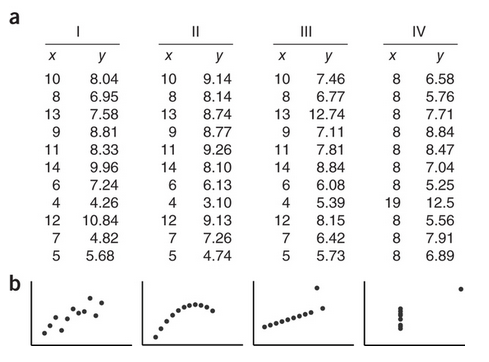
\includegraphics[scale=0.8]{anscombes_quartet.png}
	\caption{Anscombe's Quartet \cite{Shoresh2012}}
\end{figure}
%%%%%%%%%%%%%%%%%%

\paragraph{Tufte}
General purpose visualization techniques have evolved over the past several decades, but often simple techniques still provide the most effective solution. One of the most seminal works in information display is Edward Tufte's "The Visual Display of Quantitative Information"\cite{Tufle1983}. This work provided a summary of several different types of visualizations applied in many fields, but more importantly it set guidelines as to what makes an effective visualization.

\paragraph{Chart Junk}
Many of the key concepts of Tufte's work revolve around the idea of limiting what he called \emph{chart junk}. Chart junk refers to "useless, non-informative, or information-obscuring elements of information displays"\cite{Tufle1983}. While Tufte acknowledges that using non-data graphics can help to editorialize or provide context for the information being displayed,  it is more important to ensure that data is not distorted in order to fit an aesthetic. 

\paragraph{Data-rich Visualizations}
In addition to limiting non-data information in visualizations, Tufte makes a strong case for the value of data-rich visualizations. Data-rich visualizations are those which include all available information, providing a comprehensive view from which macro trends may emerge. In essence, perhaps at the expense of being able to read individual data points, viewing a complete data set visually may provide insight without need for mathematical analysis. One of many examples of this given in the work is the famous map of central London used by Dr. John Snow to determine the root cause of a cholera outbreak, shown in Figure \ref{fig:snowmap}. By marking the location of cholera deaths with dots and water pumps with crosses it became immediately clear that deaths were clustered around a central pump on Broad Street. Dismantling this pump quickly stopped the deaths. This provides a clear case where a simple graphical analysis proved far more efficient than mathematical computation would have been in determining a causal link.

%%%%%%%%%%%%%%%%%%
\begin{figure}
	\centering
	\label{fig:snowmap}
	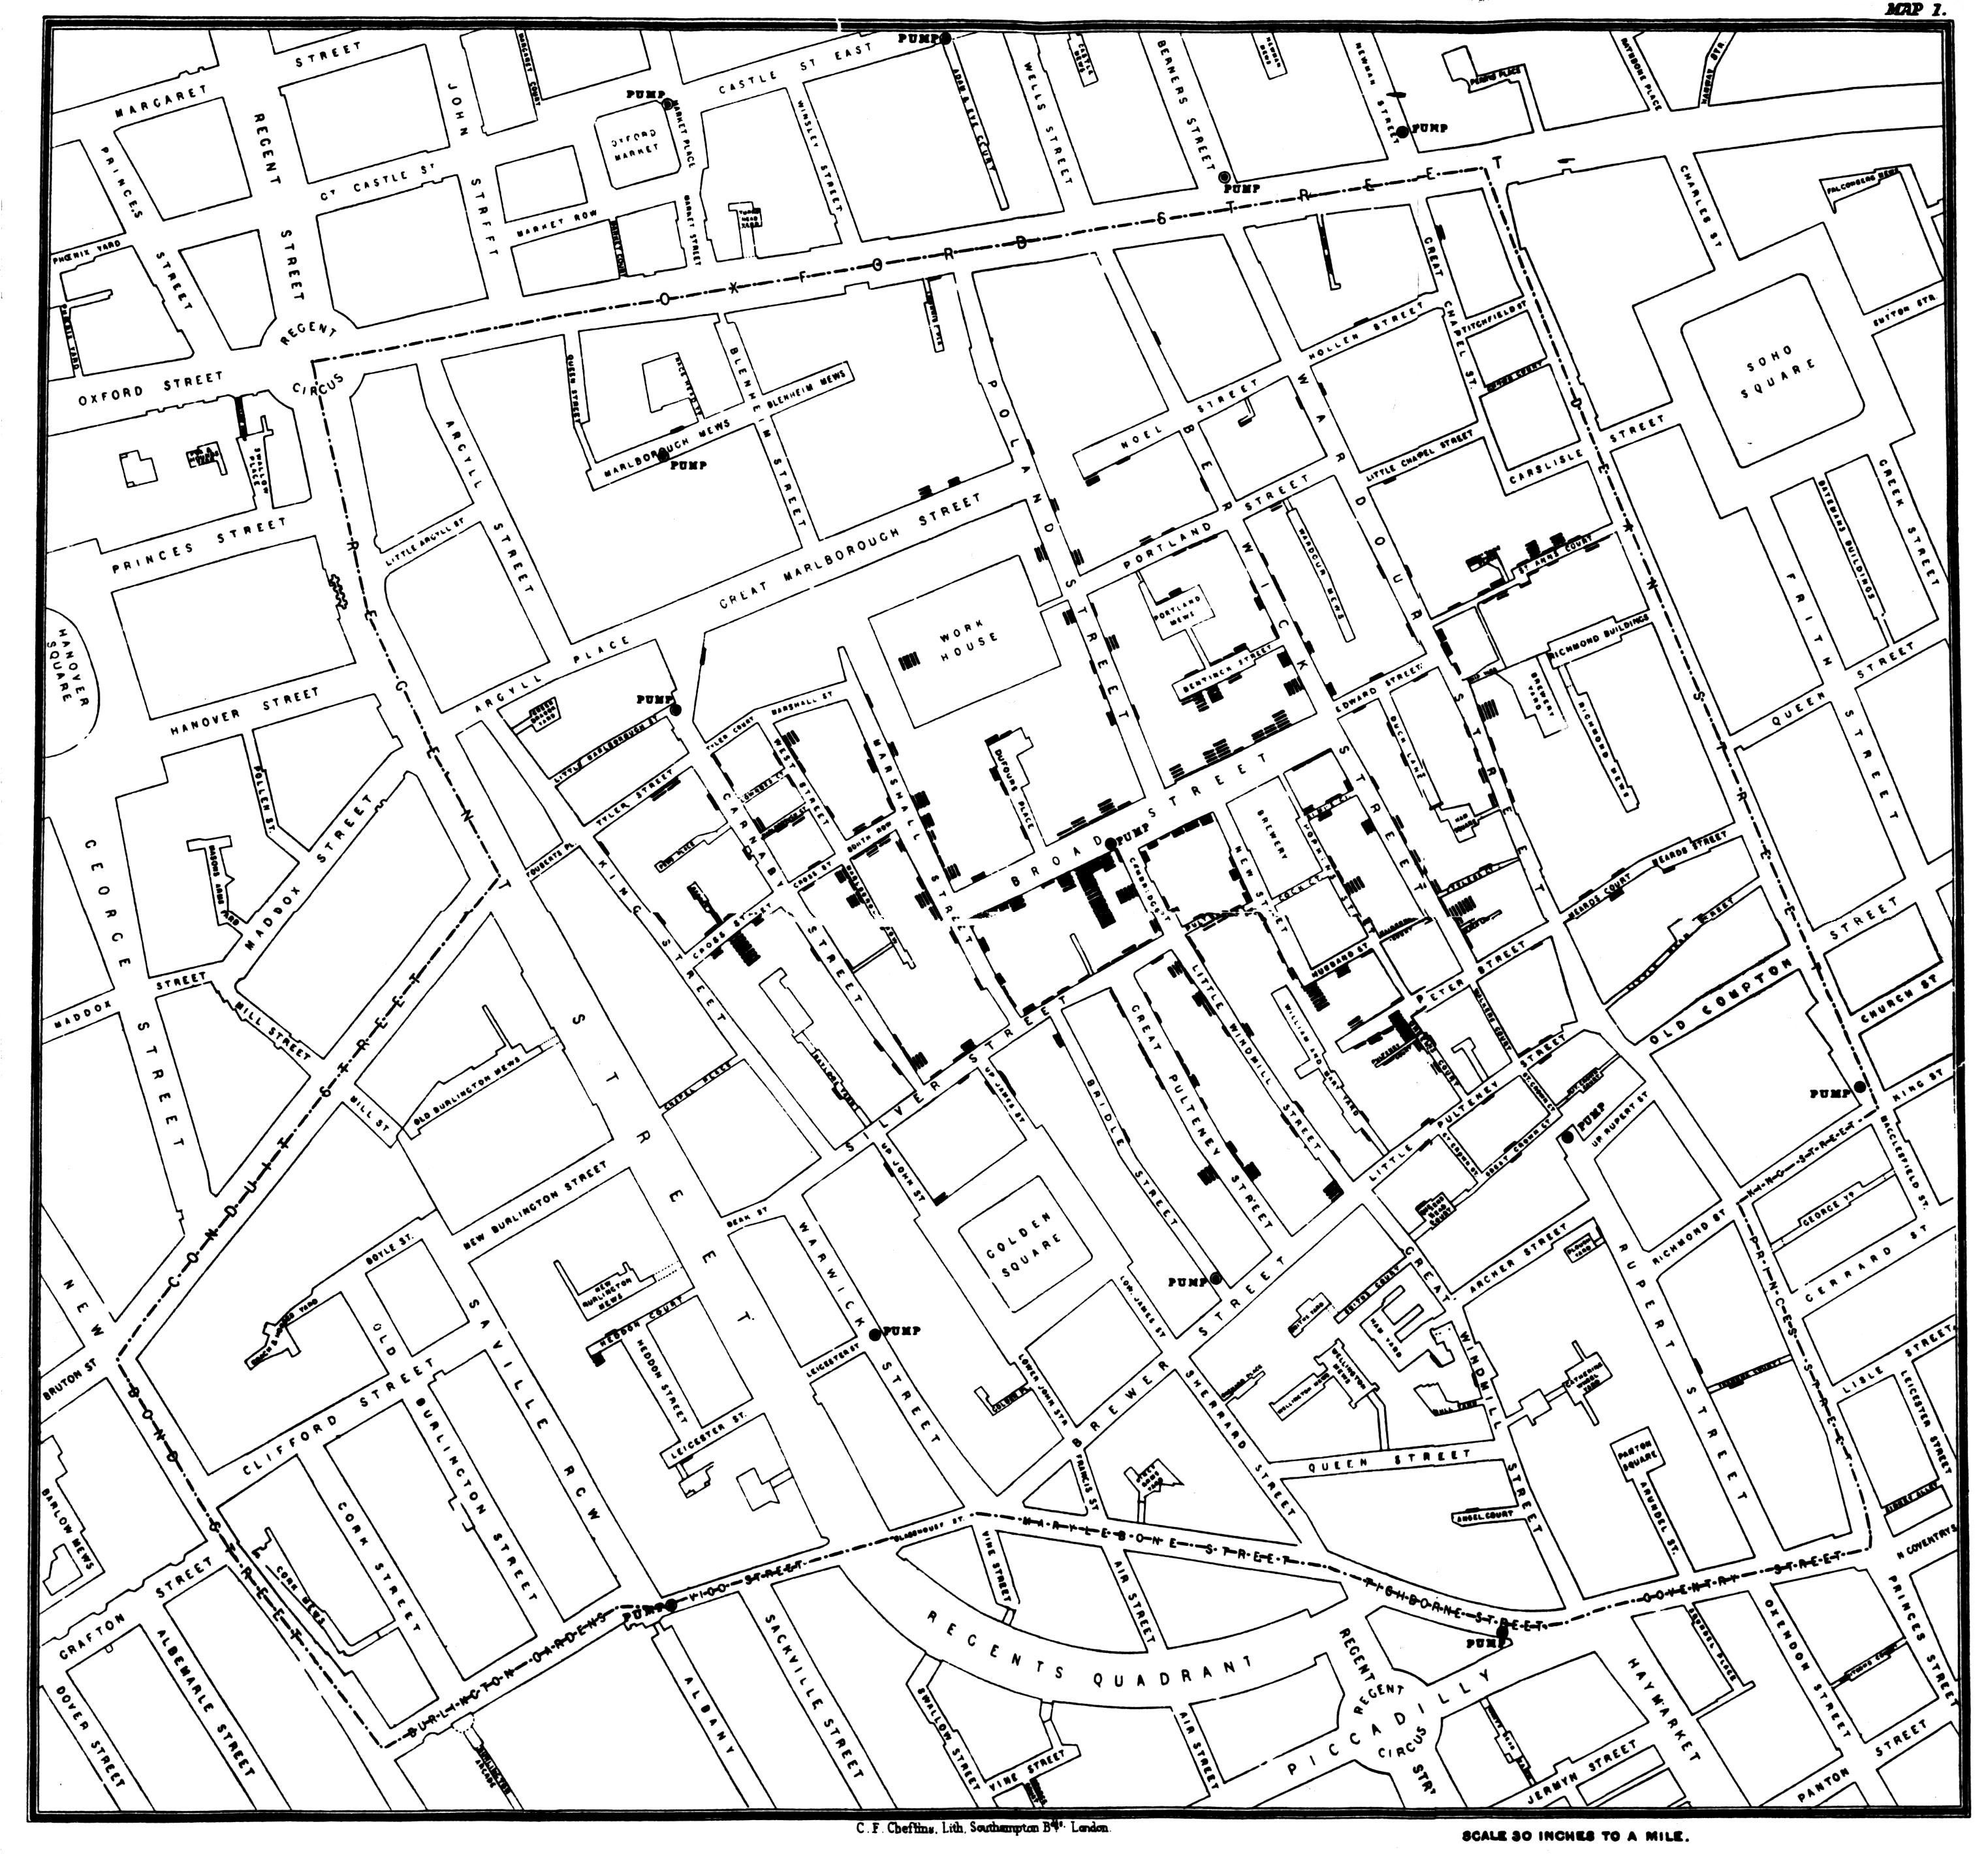
\includegraphics[scale=0.14]{jonsnowmap.jpg}
	\caption{The map used by John Snow to determine the source of a cholera outbreak \cite{Tufle1983}}
\end{figure}
%%%%%%%%%%%%%%%%%%

\paragraph{Dashboards}
A more contemporary area of work which is directly connected to digital display is the concept of a \emph{dashboard}. As defined by Stephen Few, a pre-eminent expert in this area, a dashboard is a single-screen visual display of the information required to achieve a specific set of goals. In a business context, this generally refers to key performance Indicators (KPIs). Such a dashboard is typically generated dynamically, allowing for real-time display of data trends as they occur. 

\paragraph{Dashboard constraints}
In Stephen Few's "Information Dashboard Design" \cite{Few2006} a comprehensive guide to the development of dashboards is given. In particular, specific charts and graphics are matched to appropriate use cases and perhaps more importantly, areas in which some visualizations are inappropriate are defined. Beyond being a discussion simply on visual design, interactivity is discussed. The author notes that although the capability to explore data and perform analysis is available, for monitoring purposes it is more appropriate to not allow such features. Though these analyses are often important, it is more crucial to the purpose of a dashboard to display the data in the form that the dashboard was originally designed for. To do otherwise would risk undermining the purpose, which is a focus on optimal display of key metrics.

\paragraph{Evaluation of Visualizations}
Though information visualization has been a very popular research topic for over two decades, there is little in terms of a firm framework by which the success of visualizations can be measured. A review of literature in the area \cite{Amende2010} indicates clearly that the literature is mixed on which evaluation approaches produce actionable results, and to what extent these results are accurate. The variables affecting such an analysis include both an examination of the domain in which data is being visualized, and the intended users of said visualizations. Scientific visualizations will not only demand different features than business visualizations, they will often be examined by users with very different levels of expertise. Exigent variables such as user understanding force data visualization to be examined by somewhat subjective standards in almost all cases. It is difficult to determine if there is a number of hours of productivity saved through the use of a dashboard, for example, if the application of the information therein (and therefore its results) is still heavily dependent on unpredictable external factors such as user expertise. 


\section{In-Situ Processing}
\label{sec:insitu}

\INITIAL{P}{rocessing large quantities of data} has become a common task within many organizations. Data sources such as sensor networks or click streams necessitate handling both massive quantities of information and rapid rates of change. The size of this data presents issues in the efficiency of storage solutions and there are many options for handling such problems \cite{Klasky2011}. Beyond storage, when analysis occurs on large data stores it is often necessary to apply in-situ processing rather than a more thoroughly controlled approach. In-situ analysis allows for results to be obtained quickly by ignoring much, or all, of the preprocessing that may be involved in an analysis performed on a more controlled data source. Removing preprocessing steps of course increases speed while introducing a number of potential unknown factors. Because in-situ analysis often occurs on data which is unstructured and not stored in a relational format, it fits hand in hand with analysis platforms which operate on large and unstructured data sets.

\paragraph{DFGs}
There are many platforms which are purpose built for performing analysis on large data sets, the most common of which are based on the MapReduce model of computation. Conceptually, executing an analysis task in the MapReduce paradigm simply means that the distributed computation task being performed consists of map and reduce operations which are paired to form each step of an overall computation. As more layers of map and reduce steps are added, we are left with a directed acyclic graph of operations which are chained together in a linear way, as can be seen in  Figure \ref{fig:dfg}. This figure represents two MapReduce steps, each of which is seperated by a write of the data being operated on to the file system. Systems which utilize the data flow graph model optimize these graphs by grouping together and pipelining operations in order to reduce the overhead and cost as much as possible.

%%%%%%%%%%%%%%%%%%
\begin{figure}
	\centering
	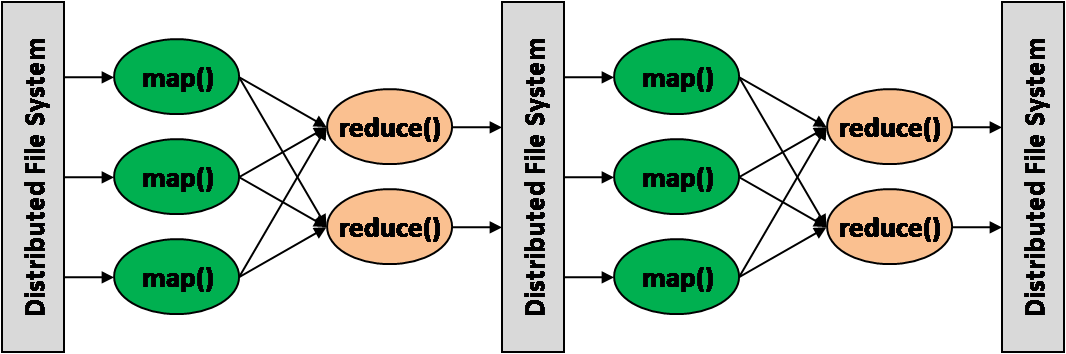
\includegraphics[scale=0.75]{Generic_DFG.png}
	\caption{A generic data flow graph \cite{Ho2008}}
	\label{fig:dfg}
\end{figure}
%%%%%%%%%%%%%%%%%%

\paragraph{Pig}
One of the more popular of the data flow graph based systems is Apache Pig \cite{Gates2009}. Pig consists of two major components: a language, Pig Latin \cite{Olston2008a} in which Pig programs can be written, and the execution environment in which they can be run. Pig acts as a high level tool through which users can develop MapReduce applications for execution in a Hadoop environment. Pig Latin provides users with a simple syntax through which sequential operations can be defined, at which point the execution environment compiles these tasks into Map-Reduce programs for which parallel implementations have already been developed in detail within Hadoop. These sequential tasks are organized into a data flow graph which the system can optimize automatically, greatly simplifying the work of the developer. Additionally, Pig Latin has been designed with extensibility in mind. Developers can write user defined functions in Java, Python, JavaScript, Ruby, or Groovy and then call these functions directly from within a Pig Latin program. Pig was initially developed internally at Yahoo, and quickly became widely applied externally after moving to the Apache foundation a year after its initial development. 

\paragraph{Flink}
Another platform for large scale data processing is Apache Flink. While Pig Latin provides the interface through which developers can work with Pig, Flink is accessed through either a Java or Scala API. For users who are already fluent in either of these languages, this is very convenient. It allows the same extensibility as seen with Pig, where users can write custom functions for execution within an analysis program, but additionally enables the use of native Java and Scala data types. Using these data types without conversion into the key-value pair data format typical of MapReduce removes one more complication for developers and simplifies analysis programs. 

\paragraph{System Differences}
Each of these systems have specific traits related to the way their data flow graphs are generated and optimized. Generally speaking however, the graphs themselves are still functionally similar enough that we can attempt to be generic in the way that this work is applied. 

\section{Visualization of Data Flow Graphs}
\label{sec:dfgviz}

\INITIAL{D}{ata flow graph visualizations} have existed in some form for as long as data flow graphs have been used in analysis systems. However, their use is almost exclusively applied to examining meta-information such as optimization plans. Relatively little work has been done in generating visualizations which help in the understanding of data, as a supplement to the analyses themselves.

\paragraph{IBM System S}
IBM research has developed a stream processing system known as \emph{System S}, which builds processing graphs using predefined operators \cite{Gedik2008} and has included basic visualization of these graphs \cite{Pauw2010}. The visualizations show the DAG of analysis operators and indicate whether the operations have completed through colour coding. Additionally, each operator has a small widget which identifies the tuples which have been passed to or from the operator, as seen in Figure \ref{fig:systemsop}. These tuples can be highlighted in order to show specific data values, and to highlight data dependencies which exist downstream.

%%%%%%%%%%%%%%%%%%
\begin{figure}
	\centering
	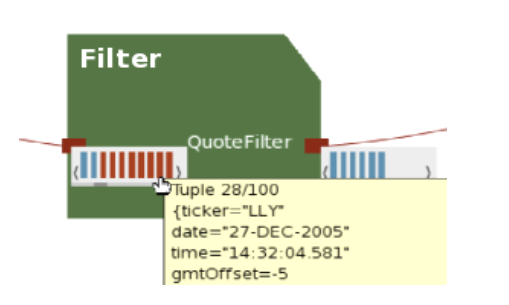
\includegraphics[scale=0.5]{SystemSOperator.png}
	\caption{An executing operator as visualized in IBM's System S 
	\cite{Pauw2010}}
	\label{fig:systemsop}	
\end{figure}
%%%%%%%%%%%%%%%%%%

\paragraph{Retrospective Debugging}
This type of visualization exists primarily to support debugging after some failure has been detected post-analysis. It can be seen in Figure \ref{fig:systemsop} that there are only ten tuples visible at a single time. Though this number can be expanded, this limitation is here because the envisioned use-case consists of a user scrolling through tuples to identify a single suspected problem tuple. While this is very useful for repairing a problem which is found post-analysis, in cases where this computation is very expensive or the problem is particularly unclear after a failure it may not be efficient. 

\paragraph{Lipstick}
Lipstick \cite{Amsterdamer2011}, a workflow provenance model framework built for use with Pig takes a similar approach to that of IBM. Lipstick examines the internals of modules within a data flow in order to determine dependencies between parts of a flow. This approach is used for very much the same debugging cases which are expected within System S, with the addition of an added feature allowing developers to query a dependency graph. These queries allow developers to change parameters of the tuples in the graph in order to undertake "what-if" style analyses. Beyond the analysis options introduced through the querying capabilities of Lipstick however, the added visualization features are relatively simple. Like in System S, single operations change colour to indicate status and the tuples being passed to and from operations are identified. In this case the key difference is that the widget for selecting single tuples from System S is replaced with a simple integer iindicating the quantity of tuples moving through a flow. The exploratory capabilities here are left for queries made against the graphs generated in Lipstick.

\paragraph{Flink Plan Visualizer}
The approach taken by Flink in visualizing the execution of a job is focused less on the provenance on data and operations and more on the organization of the execution plan as decided by the internal optimizer. Depending on the input sizes and other variable factors in a job, the same program may be executed very differently so that optimal performance can be achieved. Because the development API and the way that programs are executed are independent of one another, it is important that a developer have a mechanism through which they can see the execution order as determined by the optimizer. This is provided through the Flink execution plan visualizer \cite{ApacheSoftwareFoundation2014}, which developers can access through their browsers. A form is provided in which users can submit the execution plan in a JSON format (easily extracted from a running job through the development API), at which point it will be neatly rendered on their screen in a format similar to the example shown in FIgure \ref{fig:flinkplan}.

%%%%%%%%%%%%%%%%%%
\begin{figure}
	\centering
	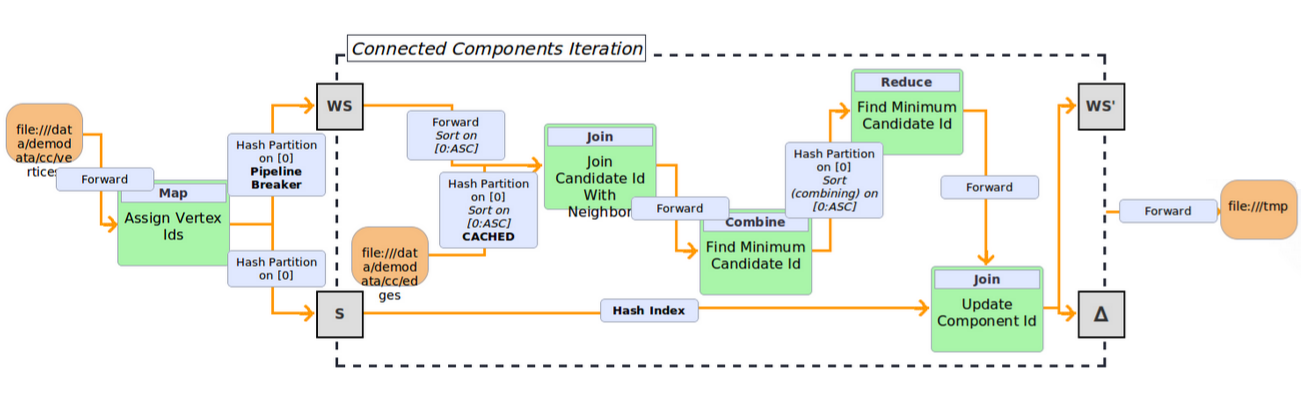
\includegraphics[scale=0.4]{flink_plan.png}
	\caption{An execution plan as seen in the Flink execution plan visualizer	\cite{ApacheSoftwareFoundation2014}}
	\label{fig:flinkplan}	
\end{figure}
%%%%%%%%%%%%%%%%%%



\cleardoublepage

\chapter{Visualizations}
\label{sec:visualizations}
\INITIAL{T}{his section aims} to provide an examination of the methods used to visualize each of the most common types of data in this work. Rather than comprehensively examining all available visualizations, focus will be placed on those data types and structures which are expected to be regularly encountered. These are the data types which are not only most regularly encountered in general, but are particularly applicable to the types of computation scenarios well-suited to analyses in a map-reduce context. 
 
%%%%%%%%%%%%%%%%%%%%%%%%%%%%%%%%%%%%%%%%%%%%%%%%%%%%%%%%%%%%%%%%%%%%%%%%%%%%
%%%%%%%%%%%%%%%%%%%%%%%%%%%%%%%%%%%%%%%%%%%%%%%%%%%%%%%%%%%%%%%%%%%%%%%%%%%%

\section{Numerical Data}
\label{sec:numerical_data}
\INITIAL{N}{umerical data is ubiquitous} when it comes to analysis. Almost all tasks which involve any type of computation will have some sort of summary  or statistics to display as a result. This ubiquity has led to a myriad of visualizations being developed for similar tasks, some of which have more merit than others. The key point to consider when visualizing numerical data is to determine the purpose of the visualization. 

\paragraph{Category Comparison}
Comparing data across several categories is a task which applies to many different forms of analysis. This is best accomplished through the use of a bar chart. Bar charts display discrete groupings of typically qualitative data such as months, product categories, or ages. Rectangular bars are rendered on the horizontal axis, with the bars' heights reflecting the value assigned to their respective categories. The ordering of the bars is often arbitrary, but in cases where the bars are ordered from highest to lowest incidence the resulting chart is known as a Pareto chart. This can help to reveal trends which exist on top of being used for comparison between two individual categories. In cases where the category values are non-discrete, they can be grouped into discrete bins based on semantically sensible ranges. In this case, the resulting chart is referred to as a histogram.  

\paragraph{Pie Chart}
Another option for comparing categories is the pie chart. A pie chart is a circle which is divided into wedges representing each category, where the arc length of a wedge reflects the category's assigned value. While these charts are visually appealing, and provide an obvious visual metaphor for parts of a whole, they are generally inferior to a simple bar chart. There are several scenarios in which a pie chart becomes very difficult to read accurately. Primarily, when there are many categories, or when the categories presented are of a very similar size. In such cases, it becomes very difficult to make judgments based on the angles of the various wedges \cite{Robbins2005}. An example of this is shown in Figure \ref{fig:winepie}, in which comparing the blue wedges accurately is quite difficult visually. While it is clear that they are all roughly similar, it is particularly difficult to be certain whether Pinot Grigio and Prosecco have equal quantities, or if one is greater. This could be corrected by adding numerical labels, but the necessity for written numbers implies that a chart may not be better suited to the task than a well formatted simple table. 

%%%%%%%%%%%%%%%%%%
\begin{figure}
	\centering
	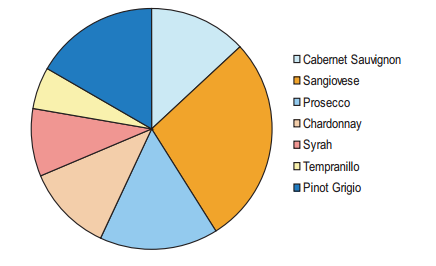
\includegraphics[scale=0.7]{pie_wine.png}
	\caption{A pie chart showing proportions of wine varieties \cite{Few2007}}
	\label{fig:winepie}
\end{figure}
%%%%%%%%%%%%%%%%%%

%%%%%%%%%%%%%%%%%%
\begin{figure}
	\centering
	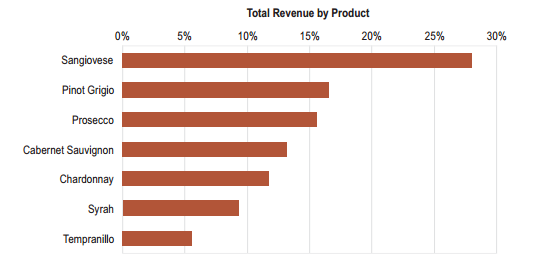
\includegraphics[scale=0.7]{bar_wine.png}
	\caption{A bar chart showing proportions of wine varieties \cite{Few2007}}
	\label{fig:winebar}
\end{figure}
%%%%%%%%%%%%%%%%%%

\paragraph{Pie Replacement}
For use in visualizing in-situ data processing in particular, we of course cannot reliably predict the proportion or in some cases number of categories in the data set. As such, it is better to assume the worst case and use a visualization which is more consistantly appropriate. Applying a percentage scale to the y-axis of a bar chart will adequately replace the visual part of whole metaphor provided by the pie chart. Aside from this, their tasks are never strongly divergent, so no other modification is necessary. Figure \ref{fig:winebar} visualizes the same data as seen in Figure \ref{fig:winepie}, using a bar chart rather than a pie. In the bar chart, the percentages are very clear and the comparison is much less ambiguous.

\paragraph{Correlation}
One of the visual analysis tasks which is best suited to human analysis is the assessment of correlation between variables. In a scenario where a data set exists with two variables, we can place each variable along an axis and mark each record as a coordinate point. Such a chart is known as a scatter plot, and suggests correlation (or lack thereof) based on the pattern of points drawn on the plot. In cases where the drawn points slope from the bottom left to the top right of the chart area, we can infer that there is a positive correlation between the two variables. Likewise, a slope from top left to bottom right implies a negative correlation. A line of best fit can be drawn on top of the scatter plot in cases where the slope is not immediately clear, or simply for clarification. 

\paragraph{Non-linear Relationships}
While seeing these positive and negative correlations is useful, it is possible to calculate them using simple methods. An even more powerful application of scatter plots is in identifying non-linear relationships between variables. For example, clusters of points are much more easily detected visually in a scatter plot than they would be through the application of statistical methods in the context of an exploratory analysis.

\paragraph{Trends} 
When examining linear trends in cases where there is a strict ordering of values on one axis, it makes sense to use a line chart. In particular, this is helpful for determining whether there is an increase or decrease in the slope of the line between individual points and through this if there is some causal relationship. Often, in cases where the trend over all data points is more important than any individual measure, sparklines can be applied. Sparklines consist exclusively of the line portion of the chart, and do not normally include axes and labeling. This is generally a design choice, and can be useful in the design of dashboards and other data-rich displays. Because of the ad-hoc nature of the analyses with which we are concerned, normal line charts will be assumed to have subsuming applicability.  

\paragraph{Summary Statistics}
There are some cases where a visualization more complex than a simple table is unnecessary and perhaps even ill-suited. When there is only a single value resulting from some aggregation, or there is nothing useful to compare resulting values to, for example. In addition, it may be the case that an analysis is complex enough that a visualization serves to further complicate understanding of the data rather than enhancing understanding. In such scenarios, it often makes sense to simply display the values on their own in comparison with other useful visualizations.

%%%%%%%%%%%%%%%%%%%%%%%%%%%%%%%%%%%%%%%%%%%%%%%%%%%%%%%%%%%%%%%%%%%%%%%%%%%%
%%%%%%%%%%%%%%%%%%%%%%%%%%%%%%%%%%%%%%%%%%%%%%%%%%%%%%%%%%%%%%%%%%%%%%%%%%%%

\section{Text Data}
\label{sec:text_data}
\INITIAL{O}{often text data is paired} with some form of numerical summary, and in many cases there is no need for a specific type of visualization for this scenario. This could be true for a data set with products and sales numbers for example, where the product names could easily be switched with an integer key and no analysis value would be lost. However, when there is semantic value which can be extracted from the text we can apply more specific techniques. Particularly, this is true if if we can present the text data itself in such a way that a viewer can assess the basic features of the data more quickly by reading the text than by using a numerical approach.

\paragraph{Word Clouds}
The most commonly encountered form of text visualization is a word cloud. Word clouds are a specific form of weighted list which were largely propagated through early blogs and websites as a common feature for exploring tags on posts. There are some examples of these visualizations appearing earlier in printed form \cite{Deleuze1987}, but these are generally not for practical analysis purposes. Word clouds can be used to either summarize the frequency with which items occur, or as a categorization method. In a frequency analysis, words within the cloud have their sizes or colours scaled to reflect their associated frequency. Categorization is applied mainly for navigational purposes, with word sizes scaling to the number of subcategories they encompass. Word clouds are often considered sub-optimal for many use cases because they remove context from the analysis and leave too much extraneous information. They still however prove quite practical for identifying flaws or unexpected features of data sets, if not for analysis. 

%%%%%%%%%%%%%%%%%%
\begin{figure}
	\centering
	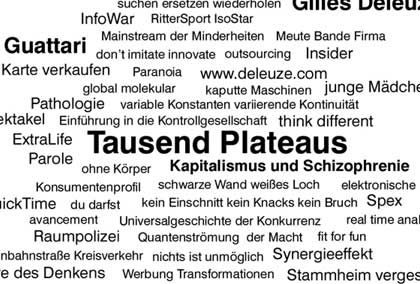
\includegraphics[scale=0.7]{tausend_plateaus_tagcloud.jpg}
	\caption{A word cloud as presented in "Tausend Plateaus: Kapitalismus und Schizophrenie" \cite{Deleuze1987}}
	\label{fig:wordcloud}
\end{figure}
%%%%%%%%%%%%%%%%%%

\paragraph{Phrase Nets}
Phrase nets \cite{VanHam2009} represent data to some extent in the same fashion as a word cloud, with the size and colour of a word representing it's frequency in the text overall. The added benefit of a phrase net is that it also shows the relationship between words, providing greater context in later stage analyses. Rather than words floating on their own, they are connected by arrows in a directed graph. The arrows are formed based on a predefined relationship between the two and weighted in the same fashion as the words themselves, based on the frequency with which the relationship occurs. Figure \ref{fig:phrasenet} shows a phrase net built using the old testament, which connects two words X and Y based on occurences of the phrase "X of Y" in the text. The obvious complication introduced in this approach is the requirement for a pre-defined relationship. Some simple relationships can be assumed to exist in most text data sets, but similar to a list of stop words it is likely that these relationships will become less useful the more commonly occurring they are. In such a case, we need to obtain a more useful relationship either through user input or some kind of natural language processing techniques. Neither case is particularly well suited for in-situ analyses, requiring significant knowledge of the data at hand or potentially complex meta-analysis respectively. 

%%%%%%%%%%%%%%%%%%
\begin{figure}
	\centering
	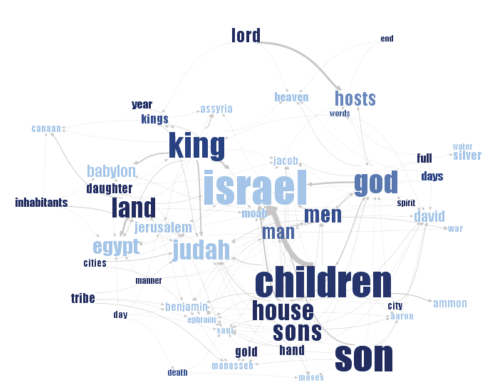
\includegraphics[scale=0.7]{phrase_net.png}
	\caption{A phrase net visualizing "X of Y" in the old testament \cite{VanHam2009}}
	\label{fig:phrasenet}
\end{figure}
%%%%%%%%%%%%%%%%%%

\paragraph{Word Trees}
A somewhat more precise visualization of text data is the word tree\cite{Wattenberg2008}. Given a specific pre-selected word, a word tree visualizes the connections that this root word has to other words in different sentences or phrases. As seen in Figure \ref{fig:wordtree}, a branch is drawn from the root word to each word which immediately follows it in the original data. Likewise, from each of these words the possible children are shown given the prior two words in a phrase. Each word in this tree is drawn at a larger size based on the number of times it follows the previous word. This provides much more context for analyzing an individual word very quickly, particularly in cases such as sentiment analysis where the tone of branching phrases and their weights can quickly identify positive or negative emotion in the data set. A word tree also offers the possibility of interaction, as a user can click any of the child nodes and generate a new tree based on this word. The specificity of this visualization also introduces technical challenges and practical issues for in-situ analysis; in particular the initial input from a user and interactivity (in cases where this is implemented). The initial input from a user implies that some knowledge of the data set's details are known beforehand to the extent that specific phrases or words are of interest and have been identified, which is likely not the case. More importantly, the method through which these trees are dynamically drawn based on the selection of any node requires re-drawing of the tree and the generation of a new set of sub-trees. This begins to shift the implementation problem from visualization and exploration towards NLP and analysis, and depending on the size of the data set in question introduces a not insignificant overhead in terms of processing. 

%%%%%%%%%%%%%%%%%%
\begin{figure}
	\centering
	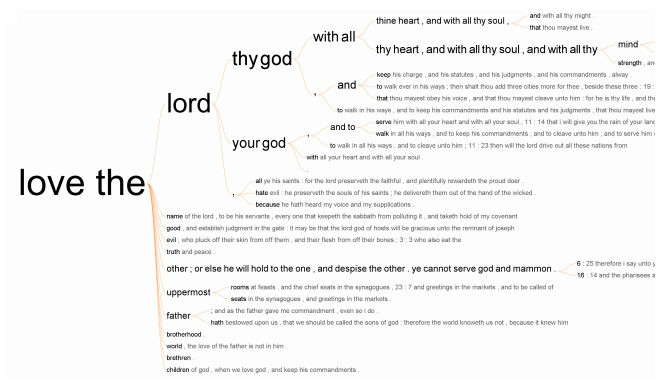
\includegraphics[scale=0.7]{word_tree.png}
	\caption{A word tree visualizing occurrences of "love the" in the King James Bible \cite{Wattenberg2008}}
	\label{fig:wordtree}
\end{figure}
%%%%%%%%%%%%%%%%%%



%%%%%%%%%%%%%%%%%%%%%%%%%%%%%%%%%%%%%%%%%%%%%%%%%%%%%%%%%%%%%%%%%%%%%%%%%%%%
%%%%%%%%%%%%%%%%%%%%%%%%%%%%%%%%%%%%%%%%%%%%%%%%%%%%%%%%%%%%%%%%%%%%%%%%%%%%

\section{Graph Data}
\label{sec:graph_data}
\INITIAL{G}{raph and network} datasets are frequently topics of interest for analysts. Particularly, the subset of graph theory known as network theory provides many methods through which analysts can discover useful features of graphs. Network theory assumes that a graph is a representation of asymmetric relationships between discrete objects (as opposed to more abstract definitions as applied in graph theory generally) and has many practical real-world applications. Any area in which real networks between objects occur, such as links in computer networks, social networks, narrative connections in writing,  or even molecular networks in biology, can provide a myriad of use cases for analyses that fall under network theory. 

\paragraph{Graphs in DAG Systems}

\paragraph{KONECT}
The KONECT project \cite{Kunegis2013} at the University of Koblenz-Landau has collected a large set of network datasets and provided tools for their analysis. Their collection demonstrates that a very large number of heterogeneous data sets can be modeled as networks, and further that a generic set of analyses can be applied to these data sets if they are represented in a unified way. Though there is a taxonomy of networks based on their respective features (directed/undirected, weighted/unweighted, etc.) the vast majority of analyses are similar if not identical, and differences typically only affect the way in which analysis is performed rather than the analysis result format. Likewise, each of these analyses can be visualized in a straightforward manner.

\paragraph{Distributions}
As networks are at their core build of distinct parts, many of the relevant analyses focus on the distribution of features among the nodes or edges therein. Generally, these analyses consist of generating distributions of features across nodes or edges, and thus each can be visualized similarly. Within weighted graphs, the distribution of weights across edges in the graph provides a good representation of any skew or trends in the weighting. An example of this can be seen in Figure \ref{fig:edgeweight}. In cases where the graph is being generated during the execution of some task rather than being provided as input, such distributions can be visualized as a temporal distribution, representing a rate of change in the overall number of edges or nodes at specific points in time, such as can be seen in Figure \ref{fig:temporaldist}. Of course, these distribution analyses can be focused on other objects within the network, for example degree distributions rather than edge weight distributions. Each type of distribution will reveal some insight into either the nodes or edges of the graph. 

\paragraph{Cumulative Degree Distribution}
While distributions focus on simple aspects of a network's structure, more complex details can be extracted from the same basic data. For example, a cumulative degree distribution can be extracted to identify the probability that a randomly selected node will have a degree larger than some integer \emph{n}, as a function of \emph{n}. Such a distribution can be seen in Figure \ref{fig:cumdist}. This figure demonstrates that even as we move to more complex forms of analysis, the structure of the output data is still well suited to our basic forms of visualization. 

%%%%%%%%%%%%%%%%%%
\begin{figure}
	\centering
	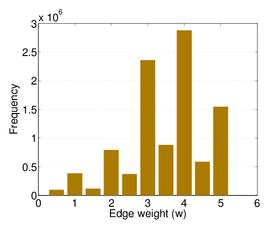
\includegraphics[scale=1.0]{edgeweight_example.png}
	\caption{A visualization of edge weight distribution \cite{KONECT}}
	\label{fig:edgeweight}
\end{figure}
%%%%%%%%%%%%%%%%%%

%%%%%%%%%%%%%%%%%%
\begin{figure}
	\centering
	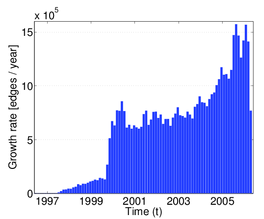
\includegraphics[scale=1.0]{temporaldist_example.png}
	\caption{A temporal visualization of edge growth \cite{KONECT}}
	\label{fig:temporaldist}
\end{figure}
%%%%%%%%%%%%%%%%%%

%%%%%%%%%%%%%%%%%%
\begin{figure}
	\centering
	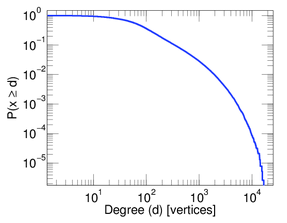
\includegraphics[scale=1.0]{cumdist_example.png}
	\caption{A visualization of cumulative distribution \cite{KONECT}}
	\label{fig:cumdist}
\end{figure}
%%%%%%%%%%%%%%%%%%

\paragraph{Layout}
As graphs are of course a form of structural data, visualizing the structure itself is intuitive. With very small graphs this is easy to do, but as graphs grow many problems present themselves. The most obvious issue is the size itself; a graph featuring ten million nodes will be impossible to visualize in a legible way unless it has very particular features which are accounted for beforehand and visualized accordingly. In the case of even relatively small graphs, it is usually necessary to have some kind of structural information about the graph so that node placement can be handled in a sensible way during visualization. Node placement has to consider not only visibility for users, but also semantic issues such as neighbor proximity and edge overlap. Some generic methods for such problems exist, such as force-directed flow algorithms \cite{Didimo2011}, but it is difficult to predict their efficacy in ad-hoc scenarios where the graph's structure is unknown.
 

%%%%%%%%%%%%%%%%%%%%%%%%%%%%%%%%%%%%%%%%%%%%%%%%%%%%%%%%%%%%%%%%%%%%%%%%%%%%
%%%%%%%%%%%%%%%%%%%%%%%%%%%%%%%%%%%%%%%%%%%%%%%%%%%%%%%%%%%%%%%%%%%%%%%%%%%%

\section{Summary}
\label{sec:vis_summary}
\INITIAL{L}{ooking at the scenarios} presented in the previous section, it becomes clear that the vast majority of visualization scenarios which would be encountered during exploratory or in-situ processing can be handled using very basic tools. Specifically, these include bar charts, line charts, scatterplots, and simple mutations of each. 

%%%%%%%%%%%%%%%%%%%%%%%%%%%%%%%%%%%%%%%%%%%%%%%%%%%%%%%%%%%%%%%%%%%%%%%%%%%%%%%%%

\begin{table}[]
\centering
\caption{Table showing pattern categories and applicable visualizations}
\label{tbl:patterns}
\begin{tabular}{llllll}
\multicolumn{1}{l|}{}                & Numerical     & Text      & Network        & Hierarchical   \\ \hline
\multicolumn{1}{l|}{Bar Chart}       & \checkmark    &           &                &                \\
\multicolumn{1}{l|}{Pie Chart}       & \checkmark    &           &                &                \\
\multicolumn{1}{l|}{Line Chart}      & \checkmark    &           &                &                \\
\multicolumn{1}{l|}{Scatter Plot}    & \checkmark    &           &                &                \\
\multicolumn{1}{l|}{Word Cloud}      &               & \checkmark&                &                \\
\multicolumn{1}{l|}{Word Tree}       &               & \checkmark&                &                \\
\multicolumn{1}{l|}{Phrase Net}      &               & \checkmark&                &                \\
\multicolumn{1}{l|}{Network Diagram} &               &           & \checkmark     &                \\
\multicolumn{1}{l|}{Tree Map}        &               &           &                & \checkmark     \\
\multicolumn{1}{l|}Text Output       & \checkmark    & \checkmark&                &   
\end{tabular}
\end{table}
%%%%%%%%%%%%%%%%%%%%%%%%%%%%%%%%%%%%%%%%%%%%%%%%%%%%%%%%%%%%%%%%%%%%%%%%%%%%%%%%%
\cleardoublepage

\chapter{MapReduce Patterns}
\label{sec:mapreducepatterns}
\INITIAL{T}{here are many scenarios} in which MapReduce can be applied. Because this work is meant to applicable to any MapReduce job, example cases must be selected in order to cover a varied range of analyses and data types. In this case, the analyses chosen attempt to cover the major MapReduce pattern categories as presented in the text "MapReduce Design Patterns" \cite{Miner2012}. Of course, in addition to the analysis itself the type of data being visualized is key. As such, these design patterns have been chosen in order to represent the most essential functions of MapReduce analysis, and thus the widest applicable range of input data sets.

%%%%%%%%%%%%%%%%%%%%%%%%%%%%%%%%%%%%%%%%%%%%%%%%%%%%%%%%%%%%%%%%%%%%%%%%%%%%
%%%%%%%%%%%%%%%%%%%%%%%%%%%%%%%%%%%%%%%%%%%%%%%%%%%%%%%%%%%%%%%%%%%%%%%%%%%%
\section{Summarization Patterns}
\label{sec:summarization}
\INITIAL{N}{umerical aggregation tasks} across groupings in a data set are the most common tasks which are encountered in MapReduce analysis programs. This base grouping of data is of course one of the most core functions of the MapReduce paradigm, and thus is often the most straightforward and commonly encountered type of analysis. Because of the simplicity of summarization tasks, they are frequently the first form of analysis performed in the exploration of a new data set. This makes summarization patterns a crucial, albeit straightforward, point of focus for any work concerning the evaluation of unknown factors in data.

\paragraph{Numerical Summary}
Numerical summarization is a general pattern for calculation aggregate statistical values across groupings in a data set. Most data sets will be too large for a human to be able to extract meaningful patterns from viewing individual records. Hence, when we are dealing with data that can be grouped by fields in a semantically meaningful way and can be sensibly aggregated or counted we can summarize in hopes of revealing insight. This pattern is analagous to performing an aggregation after a group by expression in a SQL-like context.

\paragraph{Inverted Index}
Inverted indexes are often constructed in scenarios when it is useful to associate some key term with a set of related results within a dataset. This serves to improve search speed by eliminating the need to examine each possible result in a large data set. It does this by pre-restricting the potential results to those which are known to be associated with the search term provided. This differs structurally from the numerical summarization pattern in that the result will be a set of record identifiers mapped onto some search keyword, rather than the relatively simpler group identifier-statistic pairs provided by numerical summarization. Though the actual implementation of the analysis differs, the information which would be useful for basic analysis remains very similar. Namely, the most crucial information here would be the number and nature of results associated with each keyword. This is generally identical to the previous visualization scenario, if we consider the dataset to be visualized as a set of keywords and associated statistical result set metadata (Number of results, average result size, etc.).  

\paragraph{Counting}
Semantically, counting problems could be considered a subset of numerical summarization. In scenarios where we require only a simple count or summary of a specific field, we could output the key of a record with a count of one and then reduce to generate a final count. The counting pattern instead utilizes the internal counting mechanism of our mapreduce framework to render the use of a reduce or summation stage unnecessary. One can simply create a counter with the ID of the field to be counted and increment by one until logging the result before the end of the execution. An example of a case where this is more efficient than a normal numerical summarization is the classic word count example. As the differences between this pattern differ in implementation rather than goal, the visualization scenarios are likewise identical to those found with numerical summarization. 

\section{Filtering Patterns}
\label{sec:filtering}

\INITIAL{F}{iltering patterns} are primarily concerned with understanding a specific part of an overall data set. As such, all filtering patterns are defined by the fact that they do not alter records in the data set, and that they each return a subset of the original data set. This can be considered analogous to search tasks, in that a set of relevant records is returned based on some provided criteria. All filtering tasks require that data be organized into discrete records.

\paragraph{Sampling}
In the context of map-reduce problems in particular, filtering is very useful for sampling. In situations where the data set to be analyzed is too large for processing in full, sampling methods can provide representative subsets. In some cases there are analysis based reasons to perform sampling; such as separating data into training and testing sets for machine learning algorithms. While this alone makes filtering an interesting use case, sampling is of specific interest for this work due to it's frequent application in exploratory analyses. When testing of an analysis job is performed on a large unknown data set, it is intuitive to simply select an arbitrary subset of records to analyze for debugging purposes. This likely provides a skewed view of the data, and an appropriately sampled data set will provide a more representative view of the task at hand. 

\paragraph{Filtering}
Filtering itself serves as an abstract pattern for the many different types of filtering that can occur in an analysis job. This is of course the most basic filtering function, wherein a subset of the records in a data set are removed based on whether they are of interest or not. In processing systems such as Flink, the purpose is very typically to collect a large sum of data in one place. Simple filtering can serve to either pare some unnecessary data from this sum, or focus on a small set of records or attributes which are particularly important.

\paragraph{Bloom Filtering}
Bloom filtering performs much the same task as basic filtering, but with added control in the method through which records are selected for filtering. When applying a bloom filter we extract a feature from each record, and compare that value to a set of values represented by the filter. The primary difference between this and standard filtering are that the decision to filter a given record is determined by the result of a set operation against our filter values. For this approach to be relevant, we must have extractable features which can be compared to the set of filter values, and these filter values must be predefined. It is possible when applying a bloom filter that some records will not be filtered out when they should have been, so they should only be used in scenarios where false positives are acceptable. Such a scenario could occur when prefiltering before performing a more thorough, and much more expensive, robust filtering.

\paragraph{Top N}
Performing a top N filter on a data set is of course distinct in that the size of the output data set is known before filtering occurs. Functionally, this is of course very similar to the previous two filtering methods. The application however differs in that there is a clear semantic application of this filter, the collection of outliers. In map-reduce settings this can be a particularly interesting problem as the typical method for accomplishing such a task in another context generally involves sorting the items in a data set, an extremely involved task using MapReduce. This provides additional information about our output, as we can infer that the output of a top N filter will be significantly smaller than the original data set; otherwise a total ordering is often a more suitable approach.

\paragraph{Distinct}
Filtering for distinct records is of course self-explanatory in meaning. There are several applications for such a filter, the most common of which is most likely removing duplicate records. In collecting data sets, duplication of records is a frequent data quality issue which can both add unnecessary processing time and skew analysis results. 


\section{Data Organization Patterns}
\label{sec:dataorganization}
\INITIAL{D}{ata organization} problems can present themselves in many ways, and have a wide variety of motivations behind them. With respect to big data problems in particular, the way that data is partitioned, sharded, or sorted can have serious implications for performance. If we consider in-situ processing in particular, there are many cases where data will need to be restructured for further analysis beyond that which is performed in the map-reduce context.

\paragraph{Structured to Hierarchical}
The structured to hierarchical pattern takes a row based data set and transforms it into a hierarchical format such as JSON or XML. Because MapReduce systems don't care about data format, hierarchical data structures can be immensely helpful in avoiding joins.

\paragraph{Partitioning}
Partitioning of course separates data into categories. This can be considered semantically similar to a summarization task without any form of aggregation, although the implementation may differ significantly. The major requirement of a partitioning job is to know in advance how many partitions should be created. This can be user provided, or derived from a prior analysis job, in which case the number of partitions may remain unknown to the user. Partitioning becomes very interesting for performance reasons when the partitions are actually sharded across different physical machines in a cluster.

\paragraph{Binning}
Binning can often be used to solve the same problems as partitioning and is very similar overall. The key difference between the two lies in implementation; binning splits data in the map phase instead of within a partitioner, eliminating the need for a reduce phase. The data structures, and therefore types of visualizations that we would want to see, in such a scenario are identical.

\paragraph{Sorting}
The total order sorting pattern is of course concerned with the order of records within a data set. 

\paragraph{Shuffling}


\section{Join Patterns}
\label{sec:joins}
It is relatively uncommon for all of the data used in a large analysis to stem from the same source. Data can originate from log files, databases, or from a sensor stream feeding directly into HDFS. While joins are simple to perform in other development environments, as is the case with SQL, often requiring only one simple command, in MapReduce environments much of the work must be performed by the developer. Because of the inherent complexity of join operations, there are several useful patterns for implementing them in MapReduce depending on what the specific needs of the scenario are. 

\paragraph{Reduce Side Join}
The simplest of the core join patterns is the reduce side join. It can be used to execute any of the basic joins seen in a standard SQL implementation (inner, left outer, right outer, full outer, antijoin, and cartesian product) and sets no limits on the sizes of data sets involved. The general use case for such a join pattern is a scenario where flexibility is desired, and a foreign key exists upon which to perform the join. In implementation terms, a mapper extracts the foreign key from each record and outputs a pair with the foreign key as a key and the entire record as a value. Then, a reducer creates temporary lists for each foreign key value across all data sets, which are then combined based on the desired join logic. This is also the most expensive of the standard join patterns because the foreign key output from the map operation means that no pre-filtering can occur. This cost can be somewhat reduced by applying a bloom filter to the records being output from the mapper. However, with such a filter the reduction in network I/O will be more useful in the case of an inner join than it will with a full outer join or antijoin; which both require all output to be sent to the reducer. 

\paragraph{Replicated Join}
In cases where only one of the data sets to be joined is large, a replicated join can be applied. In this scenario all data sets excluding the large one are read into memory, thus eliminating the need for a reduce step. The join can be performed entirely in the map phase, with the large dataset acting as input. This is of course a very strict limit set on the size of the small datasets, which is detetrmined by the size of the JVM heap. Additionally, this is really only a valid approach for an inner or left outer join where the large dataset can act as the left data set in the join. 

\paragraph{Composite Join}
The reduce phase of a join can also be eliminated for larger datasets, through the use of the composite join pattern. This method is limited however by the requirement that the datasets be organized in a specific way. Specifically, all data sets must be able to be read with the foreign key as input to a mapper, they must all have the same number of partitions, and they must be ordered by the foreign key. This is very useful in cases where inner or full outer joins are desired on structured data sources, but in cases such as in-situ processing where guarantees on features of the data set are unknown this is not a practical option for implementation.

\paragraph{Cartesian Product}
The last resort in terms of performance is of course a cartesian product. Execution a join by cartesian product is not very well suited to MapReduce, as the operation cannot be parallelized very well and requires more computation time and network traffic than another join. Nonetheless, there are occasions when there is no other option and it must be performed. The most likely candidates for such a join are text document or media analysis where discrete record fields which can be identified as foreign keys are not easily extracted. 

\section{Meta Patterns}
\label{sec:metapatterns}
\INITIAL{M}{eta patterns} encompass patterns which deal with the handling of smaller patterns rather than solving particular problems themselves. Because they don't focus on particular problems they don't yield much interesting information for visualization in and of themselves. However, they do provide insight into the way that a large analysis job might be constructed using the previously discussed patterns. This in turn demonstrates the scalability of the previously discussed patterns and by extension the scalability of visualization solutions applied to them individually.

\paragraph{Job Chaining}
Perhaps the most intuitive of the meta patterns in MapReduce is job chaining. Large problems are often not easily solved with a single MapReduce job, and thus require a series of jobs to be chained together somehow. In the simplest case, this could mean that several jobs are executed in parallel while others have their input provided by previously completed jobs. This is generally a process which relies heavily on developers, as MapReduce systems are often not equipped to handle more than one job very well and a certain degree of manual coding is required. There are some tools which are being developed to handle this issue, such as Apache's Oozie \cite{Islam2012}. Without such tools there are still several options for developers to handle such issues, such as creating  a job driver. This is very straightforward, in that a developer simply creates a generic driver task which will call the drivers for sub-tasks in turn when appropriate. Perhaps the most difficult part of such an approach is determining what the most appropriate ordering for execution is and which jobs will require input from some parent job. This approach can also be applied externally by using some kind of script to execute jobs rather than a driver class in the analysis environment itself. The JobControl and ControlledJob classes form a system for chaining MapReduce jobs in Hadoop, but for simpler applications this may be unnecessarily complicated. 

\paragraph{Chain Folding}
Chain folding provides a method through which job chains can be optimized further. Because each record can be submitted to multiple mappers and map phases are completely shared-nothing we know that each record will be assessed on its own regardless of grouping or data organization. This means that we can take the map setps of multiple jobs and combine them into a single map phase, significantly reducing I/O load stemming from data movement through the MapReduce pipeline.  

\paragraph{Job Merging}
Another method which is focused on reducing the I/O costs incurred by jobs is job merging. Job merging applies when more than one job uses the same set(s) of data during their execution. In some cases, if the data set is large enough the initial loading stage may even be the most costly portion of the analysis flow, and is divided for each job that can be merged. There are many complications with merging jobs, not the least of which are the requirements that all keys used in intermediate stages and output formats must match between jobs so that they are both operating on the same data types. A single map function can then be used to perform the tasks of map functions from both of the sub-jobs, adding a tag to output records to identify which mapper task it is associated with. Reducers can then use conditional logic to decide what kind of reduce task to perform based on the tag provided during mapper output. The reduce results can be split to separate destinations at this point for distinct processing on a presumably much smaller set of records.

\section{Summary}
\label{sec:pattern_summary}
  


\cleardoublepage

\chapter{Implementation}
\label{sec:implementation}
\INITIAL{T}{he proposed method} for implementing an in-situ visualization system is comprised of several vital parts. Although the  output visualization is key from a user perspective, there are important factors to be considered in the way that data is collected and how this method fits into the overarching analysis system. 
 
%%%%%%%%%%%%%%%%%%%%%%%%%%%%%%%%%%%%%%%%%%%%%%%%%%%%%%%%%%%%%%%%%%%%%%%%%%%%
%%%%%%%%%%%%%%%%%%%%%%%%%%%%%%%%%%%%%%%%%%%%%%%%%%%%%%%%%%%%%%%%%%%%%%%%%%%%
\section{Overview}
\label{sec:overview}
\INITIAL{T}{he core development portion of this work} is based on the classes which generate visualizations using a Flink execution plan. Firstly, there is an In-Situ Collector class which has the sole purpose of collecting data sets and/or summaries of data sets as they are run through the Flink analysis task. After data has been collected, the Visualizer can perform various visualization tasks based on the datasets which it has been provided. Figure \ref{fig:uml} shows the basic structural parts of this development. 

\paragraph{Visualization Classes}
While the aforementioned two classes perform the  bulk of the mechanical work, the visualizations themselves each require their own specialized classes which can be invoked generically from the Visualizer. For standard visualizations such as a histogram these classes largely handle the translation of data sets into a more easily digestible format which can be passed to pre-existing robust visualization libraries. In more complex and specific scenarios such as generating phrase nets, 'sketches' have been written in the Processing visualization language. These sketches can, with some minor modifications, be used within java projects and then drawn using the java swing toolkit. 

%%%%%%%%%%%%%%%%%%
\begin{figure}
	\centering
	\label{fig:uml}
	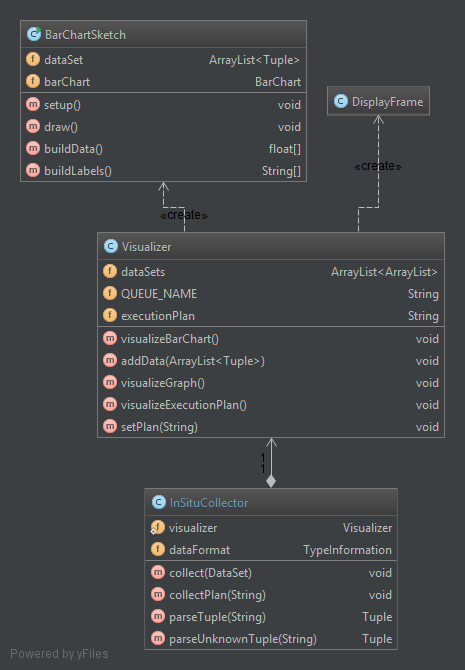
\includegraphics[scale=0.5]{uml_diagram.png}
	\caption{A UML diagram of the core classes}
	\TODO{Replace figure with updated/formatted version}
\end{figure}
%%%%%%%%%%%%%%%%%%

%%%%%%%%%%%%%%%%%%%%%%%%%%%%%%%%%%%%%%%%%%%%%%%%%%%%%%%%%%%%%%%%%%%%%%%%%%%%
%%%%%%%%%%%%%%%%%%%%%%%%%%%%%%%%%%%%%%%%%%%%%%%%%%%%%%%%%%%%%%%%%%%%%%%%%%%%
\section{Data Collection}
\label{sec:data_collection}
\INITIAL{D}{ata types in Flink} are analyzed by the optimizer to determine the most efficient execution strategies. In order to make this process simpler, Flink places limits on the types of data which can be used. There are four categories of types: General objects and POJOs, Tuples, Values, and Hadoop writeables. The handling of each of these types must of course be considered when data is being collected from an analysis graph.

\paragraph{Tuples}
Tuples are used to represent composite data sets, and are composed of a set length list of fields of various types. Tuples can include any valid Flink type as an element, including further tuples. One of the major benefits of using tuple types is the ability to use built-in functions to navigate through the tuple values. Specifically, these functions allow the selection of specific fields as the key for operations and more generally allow the navigation of tuple fields using string expressions.

\paragraph{Values}
Values are types which have their serialization and de-serialization specified manually.

\paragraph{Hadoop Writeables}
Objects which implement the Hadoop writeable interface.

\paragraph{Data Collector}
The data collector class acts as a simple addition to a pre-existing analysis program in Flink which collects data as it passes through operations. A single collector object exists for a given analysis flow, and collects data at a specific point with a single added line of code calling the collect method.

\paragraph{Collect Method}
Each time the collect method is called, it sends a new dataset to the central visualizer class. This method accepts a dataset as its sole argument and writes this dataset to memory in a format which can be read by the data collector. The data collector then reads this data into a new dataset outside of the original analysis flow's execution environment.
  
\paragraph{Data Sets}
A custom data set class exists for the use of the collector and visualizer. This class is very similar to the data set class which is native to Flink, but allows for the tracking of additional metadata which may be useful for debugging. This information could include timestamps, tags referring to specific operations in the analysis flow, or other semantically relevant information. These datasets are always initialized to contain tuple type objects. As a tuple can of course include any item of a basic type, this implementation will create a tuple of any general object in order to simplify data set operations. For example, if a single integer field is passed through the initial analysis flow, the data set generated in the visualizer will consider this as a tuple of size one which contains an integer.

\paragraph{Type Erasure}
When analysis jobs are executed, the java compiler will erase types and operate exclusively with generics. This means that when this data is extracted, some additional work is needed in order to determine a sufficient approximation of the original type for storage in a custom data set. To handle this, as each record is read into a data collector they are parsed through a set of pattern matching checks which determine the number of fields and the fields' types. Firstly, a simple line split determines the size of the tuples which should exist in the data set based on the input record. Next, each field is checked individually using the java string utilities library to determine whether they are numeric or non-numeric. Fields in each of these categories are then passed through a cascading set of conditional checks which determine their specific basic type, from least to most complex. For example, this method will attempt to parse a numeric field as an integer, and upon failure attempt to parse the field as a long. This process continues until a match is found; in the case that one is not an exception is thrown. 

%%%%%%%%%%%%%%%%%%%%%%%%%%%%%%%%%%%%%%%%%%%%%%%%%%%%%%%%%%%%%%%%%%%%%%%%%%%%
%%%%%%%%%%%%%%%%%%%%%%%%%%%%%%%%%%%%%%%%%%%%%%%%%%%%%%%%%%%%%%%%%%%%%%%%%%%%
\section{Distribution}
\label{sec:distribution}
\INITIAL{D}{istribution in analysis systems} following the general mapreduce model all operate very similarly in concept. This means that generally speaking, we can expect the dataset to be mapped into a set of key-value pairs which are then partitioned across a cluster in a uniformly distributed way. Because we may want to examine the intermediate dataset at a point prior to a reduce operation which would centralize the dataset, we must collect it piecemeal from each node in the cluster. This is achieved by sending the datasets from each node in the cluster to the visualizer for summary. 

\paragraph{Message Passing}
Message passing allows us to invoke a send message call from each in-situ data collector operating on a shard of the complete data set, and then receiving it in the visualizer. The visualizer can perform whichever operations are needed in order to merge the datasets considering the original locations and timing in order to generate useful output. 

\paragraph{Patterns?}
I'm not sure yet if a specific pattern will apply.

\paragraph{RabbitMQ}
So far arbitrary.

\paragraph{Specifics}
Implementation details such as server locale etc.

%%%%%%%%%%%%%%%%%%%%%%%%%%%%%%%%%%%%%%%%%%%%%%%%%%%%%%%%%%%%%%%%%%%%%%%%%%%%
%%%%%%%%%%%%%%%%%%%%%%%%%%%%%%%%%%%%%%%%%%%%%%%%%%%%%%%%%%%%%%%%%%%%%%%%%%%%
\section{Visualization}
\label{visualization}

\INITIAL{D}{eveloping visualizations} in software is a matter of both design and engineering. Finding an effective way to build visuals is often as important as selecting and conceptualizing the most appropriate way to convey the information at hand. In building the visualizations in this work, several languages and libraries have been applied in order to complete the work in the most effective way possible.

\paragraph{Processing}
Processing is a language which was initially developed as a teaching tool for computer programming fundamentals which utilized visual arts as a context. It was first released in 2001 as a project of the MIT aesthetics and computation group and has since evolved into a professional level tool for visual programming. The primary advantages of using Processing as a tool for the more complex portions of this work are it's ease of use, and compatibility with the rest of the development environment. As it was initially intended as a learning tool, the structure of a processing program is often very simple when compared with something similar generated using only java for example. A single program in Processing is referred to as a "sketch", referring to both the artistic nature of the language and the typical simplicity of it's application. In addition, processing code is compiled into java which simplifies the integration of the two. 

\paragraph{Libraries}
The City University of London's Graphical Information Center provides several useful libraries for performing visualization work. In particular, to aid in the development of work which utilizes processing sketches. The visualizations in this work have been built using classes from these utility libraries in the simplest of cases (such as the bar chart). In addition to providing basic visualizations in a pre-packaged format, there are some other tools such as navigational and formatting features which have been utilized in this work.  

\paragraph{Swing}
Outside of the visualizations themselves, the work of creating frames and navigation is largely handled through directly using java's swing visualization toolkit.

\paragraph{Presentation of Visualizations}
More comprehensive packaging, eventually.

\cleardoublepage

\chapter{Evaluation}
\label{sec:evaluation}

\section{Accuracy}
\label{sec:accuracy}

\section{Performance}
\label{sec:performance}

\section{Usefulness}
\label{sec:usefulness}
\cleardoublepage

\appendix 

\chapter{Implementation}

\section{My Algorithm}
\label{app:my_algorithm}
\INITIAL{T}{he following function} computes something

\paragraph{}
\begin{lstlisting}[language=C++,showspaces=false,showstringspaces=false,breaklines=true, breakatwhitespace=true]
#include <cv.h>
using namespace cv;
// your code goes here

\end{lstlisting}


%\input{saveschemadtd}
\cleardoublepage

%%%%%%%%%%%%%%%%%%%%%%%%%%%%%%%%%%%%%%%%%%%%%%%%%%%%%%%%%%%%%%%%%%%%%%%%%%%%%
%%% Bibliographie
%%%%%%%%%%%%%%%%%%%%%%%%%%%%%%%%%%%%%%%%%%%%%%%%%%%%%%%%%%%%%%%%%%%%%%%%%%%%%

%\addcontentsline{toc}{chapter}{Bibliography}
\bibliographystyle{IEEEtranSA}
\bstctlcite{IEEEexample:BSTcontrol} % load IEEE cite control entry
\bibliography{references}

\cleardoublepage

%%%%%%%%%%%%%%%%%%%%%%%%%%%%%%%%%%%%%%%%%%%%%%%%%%%%%%%%%%%%%%%%%%%%%%%%%%%%%
%%% Selbst‰ndigkeitserkl‰rung
%%%%%%%%%%%%%%%%%%%%%%%%%%%%%%%%%%%%%%%%%%%%%%%%%%%%%%%%%%%%%%%%%%%%%%%%%%%%%

\chapter*{Declaration of Authorship}

I declare that the work presented here is, to the best of my knowledge and belief, original and the result of my own investigations, except as acknowledged, and has not been submitted, either in part or whole, for a degree at this or any other university.
\linebreak
\linebreak
Formulations and ideas taken from other sources are cited as such. This work has not been published.\\
\\
\\


Berlin, 31 July 2015

\hspace*{\fill}\textbf{Jacob A. Edwards}


%%%%%%%%%%%%%%%%%%%%%%%%%%%%%%%%%%%%%%%%%%%%%%%%%%%%%%%%%%%%%%%%%%%%%%%%%%%%%
%%% Ende
%%%%%%%%%%%%%%%%%%%%%%%%%%%%%%%%%%%%%%%%%%%%%%%%%%%%%%%%%%%%%%%%%%%%%%%%%%%%%

\end{document}
